\begin{appendix}
\renewcommand{\thechapter}{M}

\titleformat{\chapter}[hang] % format chapter
{\Huge\mdseries\raggedright}
{}
{0pt}{\Huge\mdseries}

\titleformat{\section}[hang] % format section
{\huge\mdseries\raggedright}
{\thesection\hsp}
{0pt}{\huge\mdseries}

\titleformat{\subsection}[hang] % format subsection
{\Large\mdseries\raggedright}
{\thesubsection\hsp}
{0pt}{\Large\mdseries}

\setcounter{secnumdepth}{5}

\chapter{Materials and Methods}
\label{app:meth}

\pagenumbering{arabic}% resets `page` counter to 1
\renewcommand*{\thepage}{M - \arabic{page}}

\begin{multicols}{2}
[\section{Manufacturing Barcoded Hydrogel Beads}\label{app:meth_beads}]
\subsection{Required Buffers}
\label{app:meth_buffers}
Several buffers and solutions are needed for completion of the following protocols, all of which are filtered through a \SI{0.2}{\micro\metre} membrane after mixing \citep{zilionis2017}.\pms

%\Acrfull{tet}: \SI{480}{\milli\litre} of nuclease-free water, \SI{5}{\milli\litre} of \SI{1}{\molar} Tris-HCl (pH 7.0), \SI{10}{\milli\litre} of \SI{0.5}{\molar} \acrshort{edta}, \SI{5}{\milli\litre} of 10\% (v/v) Tween-20 in nuclease-free water.\pms

\begin{center}
\begin{tabular}{r|l}
	\multicolumn{2}{c}{\Acrfull{tet} buffer} \\
	\hline
	Nuclease-free H\textsubscript{2}O & \SI{480}{\ml} \\
	\SI{0.5}{\molar} \acrshort{edta} & \SI{10}{\ml} \\
	\SI{1}{\molar} Tris-HCl (pH 7.0) & \SI{5}{\ml} \\
	10\% Tween-20 & \SI{5}{\ml} \\
\end{tabular}
\end{center}
\medskip

% 4x \Acrfull{ab}: \SI{3.6}{\milli\litre} of acrylamide/bisacrylamide (\acrshort{aa}/\acrshort{bis}), \SI{2.58}{\milli\litre} of \acrfull{aa}, \SI{3.82}{\milli\litre} of nuclease-free water.\pms

\begin{center}
\begin{tabular}{m{5cm}|l}
	\multicolumn{2}{c}{4x Acrylamide/bis-acrylamide } \\
	\hline
	Nuclease-free H\textsubscript{2}O & \SI{3.82}{\ml} \\
	40\% (w/w) \Acrfull{aabis} & \SI{3.6}{\ml} \\
	40\% (w/w) \Acrfull{aa} & \SI{2.58}{\ml} \\
\end{tabular}
\end{center}
\medskip

% \Acrfull{tbset}: \SI{822}{\milli\litre} of nuclease-free water, \SI{10}{\milli\litre} \SI{1}{\molar} Tris-HCl (pH 8.0), \SI{137}{\milli\litre} of \SI{1}{\molar} NaCl, \SI{1.35}{\milli\litre} of \SI{2}{\molar} KCl, \SI{20}{\milli\litre} of \SI{0.5}{\molar} \acrshort{edta}, \SI{10}{\milli\litre} of 10\% (v/v) Triton X-100 in nuclease-free water.\pms

\begin{center}
\begin{tabular}{r|l}
	\multicolumn{2}{c}{\Acrfull{tbset} buffer} \\
	\hline
	Nuclease-free H\textsubscript{2}O & \SI{822}{\ml} \\
	\SI{1}{\molar} NaCl & \SI{137}{\ml} \\
	\SI{0.5}{\molar} \acrshort{edta} & \SI{20}{\ml} \\
	\SI{1}{\molar} Tris-HCl (pH 8.0) & \SI{10}{\ml} \\
	10\% (v/v) Triton X-100 & \SI{2.58}{\ml} \\
	\SI{2}{\molar} KCl & \SI{1.35}{\ml} \\
\end{tabular}
\end{center}
\medskip

% STOP-25: \SI{880}{\milli\litre} of nuclease-free water, \SI{10}{\milli\litre} of 1 M Tris-HCl (pH 8.0), \SI{50}{\milli\litre} of \SI{0.5}{\molar} \acrshort{edta}, \SI{10}{\milli\litre} of 10\% (v/v) Tween-20, and \SI{50}{\milli\litre} of \SI{2}{\molar} KCl.\pms

\begin{center}
\begin{tabular}{r|l}
	\multicolumn{2}{c}{STOP-25} \\
	\hline
	Nuclease-free H\textsubscript{2}O & \SI{880}{\ml} \\
	\SI{0.5}{\molar} \acrshort{edta} & \SI{50}{\ml} \\
	\SI{2}{\molar} KCl & \SI{50}{\ml} \\
	\SI{1}{\molar} Tris-HCl (pH 8.0) & \SI{10}{\ml} \\
	10\% (v/v) Tween-20 & \SI{10}{\ml} \\
\end{tabular}
\end{center}
\medskip

% STOP-10 buffer: \SI{1820}{\milli\litre} of nuclease-free water, \SI{20}{\milli\litre} of \SI{1}{\molar} Tris-HCl (pH 8.0), \SI{40}{\milli\litre} of 0.5 M \acrshort{edta}, \SI{20}{\milli\litre} of 10\% (v/v) Tween-20, and \SI{100}{\milli\litre} of \SI{2}{\molar} KCl.\pms

\begin{center}
\begin{tabular}{r|l}
	\multicolumn{2}{c}{STOP-10} \\
	\hline
	Nuclease-free H\textsubscript{2}O & \SI{1820}{\ml} \\
	\SI{2}{\molar} KCl & \SI{100}{\ml} \\
	\SI{0.5}{\molar} \acrshort{edta} & \SI{40}{\ml} \\
	\SI{1}{\molar} Tris-HCl (pH 8.0) & \SI{20}{\ml} \\
	10\% (v/v) Tween-20 & \SI{20}{\ml} \\
\end{tabular}
\end{center}
\medskip

% Denaturation solution: \SI{242}{\milli\litre} of nuclease-free water, \SI{3.75}{\milli\litre} of \SI{10}{\molar} NaOH, and \SI{4.2}{\milli\litre} of 30\% (wt/wt) Brij-35.\pms

\begin{center}
\begin{tabular}{r|l}
	\multicolumn{2}{c}{Denaturation solution} \\
	\hline
	Nuclease-free H\textsubscript{2}O & \SI{242}{\ml} \\
	\SI{10}{\molar} NaOH & \SI{3.75}{\ml} \\
	30\% (w/w) Brij-35 & \SI{4.2}{\ml} \\
\end{tabular}
\end{center}
\medskip

% Neutralization buffer: \SI{385}{\milli\litre} of nuclease-free water, \SI{50}{\milli\litre} of \SI{1}{\molar} Tris-HCl (pH 8.0), \SI{10}{\milli\litre} of \SI{0.5}{\molar} \acrshort{edta}, \SI{5}{\milli\litre} of  10\% (v/v) Tween-20, and \SI{50}{\milli\litre} of \SI{1}{\molar} NaCl.\pms

\begin{center}
\begin{tabular}{r|l}
	\multicolumn{2}{c}{Neutralisation buffer} \\
	\hline
	Nuclease-free H\textsubscript{2}O & \SI{385}{\ml} \\
	\SI{1}{\molar} Tris-HCl (pH 8.0) & \SI{350}{\ml} \\
	\SI{1}{\molar} NaCl & \SI{50}{\ml} \\
	\SI{0.5}{\molar} \acrshort{edta} & \SI{10}{\ml} \\
	10\% (v/v) Tween-20 & \SI{5}{\ml} \\
\end{tabular}
\end{center}
\medskip

 % Hybridization buffer: \SI{407}{\milli\litre} of nuclease-free water, \SI{5}{\milli\litre} of \SI{1}{\molar} Tris-HCl (pH 8.0), \SI{100}{\micro\litre} of 0.5 M \acrshort{edta}, \SI{5}{\milli\litre} of 10\% (v/v) Tween-20, and \SI{82.5}{\milli\litre} of \SI{2}{\molar} KCl.\pms

\begin{center}
\begin{tabular}{r|l}
	\multicolumn{2}{c}{Hybridisation buffer} \\
	\hline
	Nuclease-free H\textsubscript{2}O & \SI{407}{\ml} \\
	\SI{2}{\molar} KCl & \SI{82.5}{\ml} \\
	\SI{1}{\molar} Tris-HCl (pH 8.0) & \SI{5}{\ml} \\
	\SI{0.5}{\molar} \acrshort{edta} & \SI{100}{\ul} \\
\end{tabular}
\end{center}
\medskip

% QC buffer: \SI{24}{\milli\litre} of nuclease-free water, \SI{250}{\micro\litre} of \SI{1}{\molar} Tris-HCl (pH 8.0), \SI{500}{\micro\litre} of \SI{0.5}{\molar} \acrshort{edta}, \SI{250}{\micro\litre} of 10\% (v/v) Tween-20, and \SI{25}{\milli\litre} of \SI{2}{\molar} KCl. \pms

\begin{center}
\begin{tabular}{r|l}
	\multicolumn{2}{c}{QC Buffer} \\
	\hline
	Nuclease-free H\textsubscript{2}O & \SI{24}{\ml} \\
	\SI{2}{\molar} KCl & \SI{25}{\ml} \\
	\SI{0.5}{\molar} \acrshort{edta} & \SI{500}{\ul} \\
	\SI{1}{\molar} Tris-HCl (pH 8.0) & \SI{250}{\ul} \\
	10\% (v/v) Tween-20 & \SI{250}{\ul} \\
\end{tabular}
\end{center}
\medskip

\subsection{Producing Microfluidic Chips}
\label{app:meth_mfchips}
Silicon wafers were imprinted with an SU-8 mask by a senior lab scientist according to standard protocols \citep{xia1998}. Then, a mixture of 10 parts \acrfull{pdms} and 1 part of curing agent (SYLGARD\textsuperscript{TM}) was prepared, mixed well and degassed under vacuum for 45 min to remove air bubbles. The bubble-free \acrshort{pdms} was poured into removable \acrshort{pmma} dam surrounding every single mask on the chip at a rate of \textasciitilde{}\SI{12}{\gram} per chip, leading to an average height of \textasciitilde{}\SI{1}{\centi\metre}. The \acrshort{pdms} was cured on-chip by heating at \SI{80}{\celsius} for 2 hours. The \acrshort{pdms} slabs were then cooled and removed from the Si wafer. Inlets were punctured using \SI{1}{\milli\metre} diameter biopsy needles. A glass slide was cleaned with acetone and \acrshort{ipa} and plasmatreated together with the chip for \SI{30}{\s}. After plasma treatment, the chip was pressed onto the glass slide. Immediately after, the channels on the chip were flushed with 2\% trichloro(1H, 1H, H, 2H-perfluorooctyl)silane in \acrshort{hfe}-7500 (3M\textsuperscript{TM}) to make the channel surface hydrophobic. The chips were then baked for an additional 4 hours at \SI{80}{\celsius} and further stored with the channels taped shut.\pms

\subsection{Generating Hydrogel Microspheres}
\label{app:meth_beadgen}
Hydrogel microspheres were produced according to \cite{zilionis2017}. Emulsion oil was prepared by spiking EvaGreen QX200\textsuperscript{TM} fluorinated oil with 2\% \acrshort{temed} (v/v). The emulsion oil was fixed into a CETONI 290N neMESYS syringe pump and connected to the hydrogel bead generation chip using \SI{1}{\mm} diameter tubing. The following monomer mix prepared was loaded into a syringe, with a thin layer of \acrshort{hfe} to nullify dead volume, and the syringe was similarly fixed into the syringe pump and connected to the chip.\pms

\begin{center}
\begin{tabular}{r|l}
	\multicolumn{2}{c}{Monomer Mix} \\
	\hline
	\SI{100}{\micro\molar} Acrydite \acrshort{dna} primer & \SI{500}{\ul} \\
	4x \acrshort{ab} solution & \SI{250}{\ul} \\
	Nuclease-free H\textsubscript{2}O & \SI{120}{\ul} \\
	\acrshort{tbset} & \SI{100}{\ul} \\
	\acrshort{aps} & \SI{30}{\ul} \\
\end{tabular}
\end{center}
\medskip

Both the \acrshort{temed}-spiked oil and monomer mix were then pump through the microfluidic chip at the rates calculated in section \ref{sec:indrop_bhbproduction}. The resulting emulsion was collected under a layer of protective mineral oil and incubated overnight at \SI{65}{\celsius}.\pms

\begin{center}
\begin{tabular}{r|l}
	\multicolumn{2}{c}{Flow Rates} \\
	\hline
	Monomer Mix & \SI{1500}{\ul\per\hour} \\
	Oil & \SI{1461}{\ul\per\hour} \\
\end{tabular}
\end{center}
\medskip

The hydrogel beads must now be washed thoroughly to remove all traces of the oil phase. After removing the mineral and carrier oil phases, an equal volume of \acrshort{tbset} was added, and the emulsion was broken with 20\% (vol/vol) \acrshort{pfo}. The \acrshort{pfo}-phase was removed and this step was repeated until the beads appeared to be semi-transparent. After adding an equal volume of 1\% SPAN-80 in hexane, the beads were vortexed and then centrifuged at 5 000 g for \SI{30}{\s}. The top hexane layer was then removed and this step was repeated. The beads were then transferred to \SI{15}{\ml} tubes and topped off with \acrshort{tbset}. After centrifugation, the hexane traces were removed using a syringe. This step was repeated an additional 3 times, after which the beads were measured using the Python script (\ref{app:supp_python}) and stored for barcoding.\pms

\subsection{Bead Diameter Model}
\label{app:meth_model}
A blocked, I-optimal response surface design was generated for 8 samples and 2 blocks using SAS JMP. 2 out of the 8 flow combinations did not physically generate droplets, so they were omitted from the dataset, and the design was augmented with an additional 2 blocks of 3 runs each was added with the added parameter constrain that $Q_{oil} > 1.5 \times Q_{mono}$. Beyond this constraint, the monomer flow becomes too strong for the oil flow to generate a proper emulsion. Each block of runs was performed on a set of different microfluidic channels to account for variation in the chip. The 12 runs resulted in 12 batches of emulsions with various droplet sizes, which were individually washed and photographed under a microscope. A Python image analysis script (\ref{app:supp_python}) was used to calculate the bead sizes of the beads in the images. Finally, a number of different modelling approaches were tested and in-silico validated on previous data. The best model resulted from \acrshort{reml} regression estimation of independent quadratic models for diameter and bead size standard deviation on the non-averaged dataset. Sample 16 was omitted as it was an outlier. Significant model factors were selected using mixed stepwise selection. The diameter was then fixed and used as a non-linear constraint in a minimisation problem for bead standard deviation. The solution of this minimisation problem is the set of parameter combinations (flows) that will produce beads of a given diameter, and with the least possible deviation from the mean. The resulting data is shown in table \ref{table:bead_data} and visualised in figure \ref{fig:indrop_model_data}.

\subsection{Barcoding Hydrogel Beads}
\label{app:meth_splitpool}
Beads were washed three times in \acrshort{hbw}. Washing comprises filling the \SI{15}{\ml} tubes with \acrshort{hbw}, vortexing, centrifuging at \SI{15}{\g} for \SI{3}{\minute} and removing the supernatant. Per \si{\ml} of beads, \SI{0.241}{\ml} of Isothermal Amplification Buffer was added. The beads were vortexed, centrifuged at \SI{1000}{\g}, and supernatant was taken off. Due to increased ionic strenght, the \acrshortpl{hb} have now shrunk to \textasciitilde{}80\% of the original volume.\pms

\acrshortpl{hb} were then mixed into a hydrogel bead mix as follows:\pms

\begin{center}
\begin{tabular}{c|c}
\centering
	Hydrogel Bead Mix & \\
	\hline
	H\textsubscript{2}O & \SI{2.3}{\ml} \\
	\acrshort{hb} suspension & \SI{9.4}{\ml} \\
	\SI{10}{\milli\molar} \acrshortpl{dntp} & \SI{0.812}{\ml} \\
\end{tabular}
\end{center}
\medskip

The hydrogel bead mix was then aliquoted into a 96-well plate at \SI{125}{\ul} per well. The first set of barcoded primers (4 96-well plates) was then thawed, centrifuged for \SI{1}{\minute} at \SI{1000}{\g} and placed in a \acrshort{pcr} machine for denaturation (Lid at \SI{105}{\celsius}, \SI{70}{\celsius} for \SI{40}{\s} followed by \SI{4}{\celsius} for \SI{20}{\celsius}). Extra care must be taken when removing the seal to avoid cross-contamination.\pms

4 reaction plates were prepared by mixing \SI{30}{\ul} of hydrogel bead mix with \SI{13.5}{\ul} of one of the 384 primers. These plates were then incubated on heat blocks at \SI{85}{\celsius} for \SI{2}{\minute}, \SI{60}{\celsius} for \SI{20}{\minute} with a lid temperature of \SI{100}{\celsius}. During this step, the primers hybridise to the acrydite stubs in the hydrogel matrix.\pms

After the hybridisation has ended, \SI{15}{\ul} of isothermal reaction mix (prepared and stored on ice) was added to every well on the reaction plates.\pms

\begin{center}
\begin{tabular}{c|c}
\centering
	Isothermal Reaction Mix & \\
	\hline
	nuclease-free H\textsubscript{2}O & \SI{6.85}{\ml} \\
	10x isothermal amp. buffer & \SI{0.8}{\ml} \\
	Bst 2.0 \acrshort{dna} \SI{8000}{\unit\per\ml} & \SI{0.35}{\ml} \\
\end{tabular}
\end{center}
\medskip

Plates were then sealed and incubated on heat blocks at \SI{60}{\celsius} for \SI{60}{\minute} and \SI{4}{\celsius} indefinitely with a lid temperature of \SI{100}{\celsius}. During this step, the acrydite primer is extended with the barcoded primer by Bst 2.0 isothermal amplification.\pms

The plates were then cooled on ice, and \SI{40}{\ul} of STOP-25 buffer was added to each reaction well to stop the isothermal amplification reaction. The contents of all wells were pooled and wells were rinsed with an additional \SI{100}{\ul} of STOP-25. The pooled product was incubated in a rotator at 20 rpm for \SI{30}{\minute}.\pms

The half-barcoded beads now need to be washed thoroughly to remove all traces of unused primers, salts, \acrshortpl{dntp} and enzymes before the second round of barcoding can take place. The half-barcoded bead stock was centrifuged at \SI{300}{\g} for \SI{15}{\minute}, and the supernatant was collected and centrifuged again to collect all beads. The beads were then split equally into four separate \SI{15}{\ml} tubes and washed three times with STOP-10 buffer. Washing encompasses filling the tubes with STOP-10 buffer, rotating for \SI{10}{\minute} at room temperature, centrifuging at \SI{300}{\g} for \SI{3}{\minute} and removing the supernatant. The half-barcoded \acrshortpl{hb} were then washed 4 times in denaturation solution, 2 times in neutralisation buffer and finally 2 times in \acrshort{tet} buffer, after which the beads were stored in \SI{4}{\celsius} overnight for the next barcoding step.\pms

The half-barcoded beads were then washed 3 times in \acrshort{hbw}, and processed for a second round of barcoding as described above - but with the Barcode 2 primer plates instead of barcode 1 - and washed using the same washing steps. The resulting stock of barcoded beads is stored at \SI{4}{\celsius}.

\subsection{qPCR}
\label{app:meth_qpcr}
7 samples were prepared in triplicate with \SI{1.25}{\ul} of packed \acrshortpl{bhb} and incubated in the appropriate concentration of \acrshort{dtt}. At a total volume of \SI{4}{\ul} per sample, the concentration of beads in the \acrshort{dtt} mix was equal to the "concentration" of beads in a true droplet (taken as the inverse of the droplet volume per bead).\pms

\begin{center}
\begin{tabular}{c|ccc}
 Sample & Bead &  H\textsubscript{2}O & \SI{0.25}{\molar} \acrshort{dtt} \\
\hline
\SI{0}{\milli\molar} & \SI{2.75}{\ul} & \SI{1.25}{\ul} & \SI{0}{\ul} \\
\SI{10}{\milli\molar} & \SI{2.59}{\ul} & \SI{1.25}{\ul} & \SI{0.16}{\ul} \\
\SI{25}{\milli\molar} & \SI{2.35}{\ul} & \SI{1.25}{\ul} & \SI{0.4}{\ul} \\
\SI{50}{\milli\molar} & \SI{1.95}{\ul} & \SI{1.25}{\ul} & \SI{0.8}{\ul} \\
\SI{75}{\milli\molar} & \SI{1.55}{\ul} & \SI{1.25}{\ul} & \SI{1.2}{\ul} \\
\SI{100}{\milli\molar} & \SI{1.15}{\ul} & \SI{1.25}{\ul} & \SI{1.6}{\ul} \\
\SI{125}{\milli\molar} & \SI{0.75}{\ul} & \SI{1.25}{\ul} & \SI{2}{\ul} \\
\end{tabular}
\end{center}
\medskip

The beads were incubated for 30 minutes, after which they were centrifuged (\SI{5000}{\rcf}, \SI{2}{\minute}), and the supernatant was processed for \acrshort{qpcr} using ready-to-use hot-start \acrshort{pcr} mix containing FastStart Taq \acrshort{dna} polymerase, reaction buffer, \acrshort{dntp} mix with dUTP instead of dTTP, Sybr Green I dye and MgCl\textsubscript{2}.\pms

\begin{center}
\begin{tabular}{r|l}
	\multicolumn{2}{c}{\acrshort{qpcr} mix} \\
	\hline
	FastStart Taq mix & \SI{5}{\ul} \\
	Bead supernatant & \SI{2.5}{\ul} \\
	Ultra-pure H\textsubscript{2}O & \SI{1.5}{\ul} \\
	\SI{10}{\micro\molar} \acrshort{pcr} primer & \SI{1}{\ul} \\
\end{tabular}
\end{center}
\medskip

The following \acrshort{qpcr} program was used on the LightCycler 480:\pms

\begin{center}
\begin{tabular}{r|l}
	\multicolumn{2}{c}{\acrshort{ispcr} Program} \\
	\hline
	\SI{95}{\celsius} & \SI{5}{\minute} \\
	\hline
	45 cycles of: \SI{95}{\celsius} & \SI{10}{\second} \\
	\SI{72}{\celsius} & \SI{35}{\second} \\
	\hline
	Melting curve: \SI{95}{\celsius} & \SI{5}{\second} \\
	\SI{65}{\celsius} & \SI{1}{\min} \\
	\SI{97}{\celsius} & cont. \\
	\hline
	\SI{40}{\celsius} & \SI{10}{\second} \\
\end{tabular}
\end{center}
\medskip

\end{multicols}

\newpage
\begin{multicols}{2}
[\section{inDrop Optimisation}\label{app:meth_indrop_opt}]
The optimisation trials followed the same steps as the third and final protocol, which is described in greater detail \ref{app:meth_indrop}, but stopped where failure occurred either physically on the chip or molecularly by not yielding \acrshort{cdna}.

\subsection{Bead/Cell Loading Experiments}
\SI{180}{\ul} of bead stock was washed twice using \acrshort{hbw} and dissolved into \SI{300}{\ul} of 2X Lysis buffer. Beads were then loaded onto the chip, with cell flow replaced with \acrshort{pbs}. $Q_{bead}, Q_{cell}, Q\_{oil}$, were each varied around the limits of \SI[per-mode=symbol]{150}{\ul\per\hour} and \SI[per-mode=symbol]{1000}{\ul\per\hour}. Bead coverage was observed by taking pictures of the suspension in the outlet funnel, as well as of the resulting suspension on a glass slide. Cell loading trials were performed by similarly testing different concentrations of input cell suspension (\SI[per-mode=symbol]{300}{\per\ul}, \SI[per-mode=symbol]{600}{\per\ul} and \SI[per-mode=symbol]{1200}{\per\ul}. To achieve an ultra-pure bead solution, beads were run through an inDrop chip, replacing both cell and oil flow with \acrshort{tet} buffer. When dust stopped the flow, the process was stopped and continued on a fresh chip.\pms

\subsection{First Custom inDrop Trial}
\label{app:meth_first_indrop_trial}
MM074 cells were resuspended in the following master mix and co-encapsulated with lysis buffer and \acrshortpl{bhb} on the inDrop system. Final cell concentration of the master mix was \SI{600}{\ul}, and flow rates of 300, 200 and \SI[per-mode=symbol]{450}{\ul\per\hour} were used for cells, beads and oil respectively.\pms

\begin{center}
\begin{tabular}{r|l}
	\multicolumn{2}{c}{RT Mix} \\
	\hline
	5x RT Buffer & \SI{36}{\ul} \\
	40\% \acrshort{peg}-8000 in H\textsubscript{2}O & \SI{33.75}{\ul} \\
	H\textsubscript{2}O & \SI{13}{\ul} \\
	\SI{10}{\micro\molar} \acrshortpl{dntp} & \SI{12}{\ul} \\
	\SI{200}{\unit\per\ul} Maxima hRT & \SI{9}{\ul} \\
	\SI{4.29}{\molar} \acrshort{dtt} & \SI{6.3}{\ul} \\
	\SI{40}{\unit\per\ul} RNAse Inhibitor & \SI{4.5}{\ul} \\
	\SI{100}{\micro\molar} \acrshort{tso} & \SI{4.5}{\ul} \\
\end{tabular}
\end{center}
\medskip

The sample emulsions were collected, aliquoted into a 96-well \acrshort{pcr} plate and heat-cycled for reverse transcription. Half of the sample was then Exo I treated according to standard Exonuclease clean-up instructions. After a subsequent \acrshort{ispcr} using Terra polymerase, the libraries were purified using 0.6 x volume Ampure beads and Qubit-quantified.\pms

\begin{center}
\begin{tabular}{r|l}
	\multicolumn{2}{c}{Terra \acrshort{ispcr} Master Mix} \\
	\hline
	2x Terra Direct \acrshort{pcr} buffer & \SI{25}{\ul} \\
	Purified \acrshort{cdna} Library & \SI{20}{\ul} \\
	\SI{100}{\micro\molar} SMART \acrshort{pcr} Primer & \SI{2.5}{\ul} \\
	Terra \acrshort{dna} polymerase	& \SI{2}{\ul} \\
	Ultrapure H\textsubscript{2}O & \SI{0.5}{\ul} \\
\end{tabular}
\end{center}
\medskip

\begin{center}
\begin{tabular}{r|l}
	\multicolumn{2}{c}{\acrshort{ispcr} Program} \\
	\hline
	\SI{98}{\celsius} & \SI{3}{\minute} \\
	\hline
	14 cycles of: \SI{98}{\celsius} & \SI{20}{\second} \\
	\SI{65}{\celsius} & \SI{45}{\second} \\
	\SI{72}{\celsius} & \SI{4}{\minute} \\
	\hline
	\SI{72}{\celsius} & \SI{10}{\minute} \\
	\SI{4}{\celsius} & inf. \\
\end{tabular}
\end{center}
\medskip

\subsection{Second Custom inDrop Trial}
\label{app:meth_second_indrop_trial}
MM087 cells were processed using the identical master mix (cell density \SI{600}{\per\ul}) and inDrop parameters as the first trial, but split between two different polymerases for \acrshort{ispcr}. Terra polymerase was carried out as previously described, and the KAPA HiFi \acrshort{pcr} was performed as follows:\pms

\begin{center}
\begin{tabular}{r|l}
	\multicolumn{2}{c}{\acrshort{ispcr} Master Mix} \\
	\hline
	2x KAPA HiFi \acrshort{pcr} Mix & \SI{50}{\ul} \\
	Purified \acrshort{cdna} Library & \SI{30}{\ul} \\
	\SI{100}{\micro\molar} SMART \acrshort{pcr} Primer & \SI{2.5}{\ul} \\
	Ultrapure H\textsubscript{2}O & \SI{17.5}{\ul} \\
\end{tabular}
\end{center}
\medskip

\begin{center}
\begin{tabular}{r|l}
	\multicolumn{2}{c}{\acrshort{ispcr} Program} \\
	\hline
	\SI{98}{\celsius} & \SI{3}{\minute} \\
	\hline
	4 cycles of: \SI{98}{\celsius} & \SI{20}{\second} \\
	\SI{65}{\celsius} & \SI{45}{\second} \\
	\SI{72}{\celsius} & \SI{3}{\minute} \\
	\hline
	10 cycles of: \SI{98}{\celsius} & \SI{20}{\second} \\
	\SI{67}{\celsius} & \SI{20}{\second} \\
	\SI{72}{\celsius} & \SI{3}{\min} \\
	\hline
	\SI{72}{\celsius} & \SI{10}{\minute} \\
	\SI{4}{\celsius} & inf. \\
\end{tabular}
\end{center}
\medskip

\end{multicols}

\newpage
\begin{multicols}{2}
[\section{Final Custom inDrop Protocol}\label{app:meth_indrop}]
This final trial was first performed by a senior lab scientist and taken as standard protocol as it produced the most favourable library fragment size distribution. This protocol was repeated using the reduced complexity beads described in chapter \ref{ch:seq}.\pms

\subsection{Preparations}
All the microfluidic peripherals were set up before preparing the cells, as the time between resuspending the cells into the \acrshort{rt} master mix and starting cell encapsulation needs to be minimised. The \acrshort{pdms} microfluidic chip was fixed under a microscope, and a syringe was filled with oil and connected to the correct chip inlet via \SI{1}{\mm} tubing.\pms

The \acrshort{bhb} stock was centrifuged (\SI{1000}{\rcf}, \SI{3}{\minute}) and the supernatant was removed. \SI{60}{\ul} of condensed bead stock was added to \SI{940}{\ul} of \acrshort{hbw}, vortexed well and centrifuged (\SI{2000}{\rcf}, \SI{1.5}{\minute}). The supernatant was removed, and replaced with an equal volume of \acrshort{hbw} and the wash was repeated. Supernatant was removed, leaving \SI{200}{\ul} of condensed bead stock. The beads were incubated in an equal volume of 2x lysis buffer for \SI{10}{\minute} on ice.\pms

\begin{center}
\begin{tabular}{r|l}
	\multicolumn{2}{c}{2x Lysis Buffer} \\
	\hline
	\SI{1}{\molar} Tris HCl  & \SI{9}{\ul} \\
	\SI{5}{\molar} NaCl & \SI{1.8}{\ul} \\
	10\% IGEPAL & \SI{20}{\ul} \\
	Nuclease-free H\textsubscript{2}O & \SI{469.2}{\ul} \\
\end{tabular}
\end{center}
\medskip

The beads were then centrifuged (\SI{5000}{\rcf}, \SI{1}{\minute}) and supernatant was removed until \SI{75}{\ul} was left. The beads were then carefully centrifuged with a mini benchtop centrifuge to pull down beads sticking to the walls.\pms

A single cell suspension was prepared by collecting sample tissue or culture and dissociating according to appropriate protocols. 70 000 cells were distributed into a \SI{1.5}{\ml} eppendorf, centrifuged (\SI{300}{\rcf}, \SI{5}{\minute}) and the supernatant was carefully removed. Cells were washed with ice-cold \acrshort{pbs} and centrifuged (\SI{300}{\rcf}, \SI{5}{\minute}). Supernatant was taken, and the \acrshort{pbs} wash was repeated. The resulting cell pellet was resuspended in \SI{120}{\ul} of reverse-transcription master mix:\pms

\begin{center}
\begin{tabular}{r|l}
	\multicolumn{2}{c}{RT Mix} \\
	\hline
	5x RT Buffer & \SI{57.6}{\ul} \\
	\SI{10}{\micro\molar} \acrshortpl{dntp} & \SI{21.48}{\ul} \\
	\SI{200}{\unit\per\ul} Maxima hRT & \SI{14.28}{\ul} \\
	\SI{40}{\unit\per\ul} RNAse Inhibitor & \SI{7.2}{\ul} \\
	\SI{100}{\micro\molar} \acrshort{tso} & \SI{7.13}{\ul} \\
	\SI{4.29}{\micro\molar} \acrshort{dtt} & \SI{6.72}{\ul} \\
	H\textsubscript{2}O & \SI{5.59}{\ul} \\
\end{tabular}
\end{center}
\medskip

% \todo[inline]{add manufacturer's information on these enzymes}

Cells are now ready to proceed to the inDrop run.

\subsection{inDrop Run}
Cell and bead mix were pre-loaded into \SI{1}{\mm} tubing by filling a syringe with \acrshort{pbs}, connecting it to the tube, and carefully aspirating the solutions into the tube. The syringes were then fixed into a CETONI neMESYS 290N syringe pump, and tubing was connected to the correct inlet on the microfluidic chip. Similarly, the chip outlet was connected to a \SI{1.5}{\ml} eppendorf tube in a cold block.\pms

All flows were simultaneously primed at \SI{500}{\ul\per\hour} until they had all stabilised. Then, final flow rates were set as follows:\pms

\begin{center}
\begin{tabular}{r|l}
	\multicolumn{2}{c}{Flow rates} \\
	\hline
	Cell & \SI{800}{\ul\per\hour} \\
	Beads & \SI{1100}{\ul\per\hour} \\
	Oil & \SI{1200}{\ul\per\hour} \\
\end{tabular}
\end{center}
\medskip

Bead and cell loading must be monitored continuously under the microscope and can be tuned by adjusting flow rates. Care must be taken not to inflate the droplets with either component during flow adjustment. Cell encapsulation ended after cells ran out, and the resulting emulsion was redistributed into a 96-well plate at \SI{70}{\ul} of emulsion with \SI{30}{\ul} of EvaGreen QX200\textsuperscript{TM}. Reverse transcription was then carried out according to the following program:\pms

\begin{center}
\begin{tabular}{r|l}
	\multicolumn{2}{c}{\acrshort{rt} Program} \\
	\hline
	\SI{42}{\celsius} & \SI{90}{\minute} \\
	\SI{85}{\celsius} & \SI{5}{\minute} \\
	\SI{4}{\celsius} & inf. \\
\end{tabular}
\end{center}
\medskip

\subsection{Post-RT Clean-up and \acrshort{ispcr}}
\SI{150}{\ul} of droplet breaking solution was added to every well and mixed by pipetting.\pms

\begin{center}
\begin{tabular}{r|l}
	\multicolumn{2}{c}{Droplet Breaking Solution} \\
	\hline
	\acrshort{hfe} 7500 & \SI{700}{\ul} \\
	\acrshort{pfo} & \SI{300}{\ul} \\
\end{tabular}
\end{center}
\medskip

The broken emulsions were then transferred into Eppendorf \acrshort{dna} lo-bind \acrshort{pcr} tubes, and the bottom oil layer was removed and discarded. \SI{125}{\ul} of QIAGEN PB buffer was added to each \acrshort{pcr} tube, and the solution was mixed well by pipetting 15 times. The contents were transferred into a \SI{1.5}{\ml} Eppendorf tube and centrifuged (\SI{5000}{\rcf}, \SI{1}{\minute}) and the supernatant was removed. The \acrshort{cdna} was then purified using QIAGEN MinElute columns according to manufacturer's instructions. Final elution was performed in \SI{31}{\ul}, and the concentration was measured using an Invitrogen Qubit fluorometer.\pms

The purified \acrshort{cdna} library was then subjected to \acrshort{ispcr} using the following mix and \acrshort{pcr}-program.\pms

\begin{center}
\begin{tabular}{r|l}
	\multicolumn{2}{c}{\acrshort{ispcr} Master Mix} \\
	\hline
	2x KAPA HiFi \acrshort{pcr} Mix & \SI{50}{\ul} \\
	Purified \acrshort{cdna} Library & \SI{30}{\ul} \\
	\SI{100}{\micro\molar} SMART \acrshort{pcr} Primer & \SI{6}{\ul} \\
	Ultrapure H\textsubscript{2}O & \SI{14}{\ul} \\
\end{tabular}
\end{center}
\medskip

\begin{center}
\begin{tabular}{r|l}
	\multicolumn{2}{c}{\acrshort{ispcr} Program} \\
	\hline
	\SI{98}{\celsius} & \SI{3}{\minute} \\
	\hline
	4 cycles of: \SI{98}{\celsius} & \SI{20}{\second} \\
	\SI{65}{\celsius} & \SI{45}{\second} \\
	\SI{72}{\celsius} & \SI{3}{\minute} \\
	\hline
	10 cycles of: \SI{98}{\celsius} & \SI{20}{\second} \\
	\SI{67}{\celsius} & \SI{20}{\second} \\
	\SI{72}{\celsius} & \SI{3}{\min} \\
	\hline
	\SI{73}{\celsius} & \SI{5}{\minute} \\
	\SI{4}{\celsius} & inf. \\
\end{tabular}
\end{center}
\medskip

The \acrshort{ispcr}-amplified \acrshort{cdna} library was then purified with 0.6 volumes of SPRI beads according to manufacturer's instructions. Final elution was performed in \SI{17.5}{\ul} of ultrapure H\textsubscript{2}O. The library was then quantified using an Invitrogen Qubit fluorometer and quality-controlled using Agilent Bioanalyzer capillary electrophoresis.\pms

The amplified \acrshort{cdna} library was then end-tagged and strand-purified using the NEBNext Ultra \textsuperscript{TM} II \acrshort{dna} Library Prep Kit for Illumina.\pms

\end{multicols}

\newpage
\begin{multicols}{2}
[\section{Drop-ATAC Preliminary Trials}\label{app:meth_dropatac_opt}]
The preliminary \acrshort{dropatac} trials followed the same steps as the final protocol, which is described in greater detail \ref{app:meth_dropatac}, but stopped where failure occurred either physically due to emulsion destabilisation or molecularly by not yielding a \acrshort{dna} library.\pms

\subsection{Droplet Stability Trials}
Two different \acrshort{pcr} master mixes were tested by emulsifying them together with \SI{150}{\ul} of beads pre-soaked in \SI{150}{\ul} of 2x lysis buffer. No nuclei were used in these trials.\pms

\begin{center}
\begin{tabular}{r|l}
	\multicolumn{2}{c}{2x Lysis Buffer} \\
	\hline
	Nuclease-free H\textsubscript{2}O & \SI{1015.2}{\ul} \\
	\SI{5}{\molar} NaCl & \SI{72}{\ul} \\
	\SI{1}{\molar} Tris HCl  & \SI{60}{\ul} \\
	10\% IGEPAL & \SI{48}{\ul} \\
	10\% \acrshort{sds} & \SI{4.8}{\ul} \\
\end{tabular}
\end{center}
\medskip

\begin{center}
\begin{tabular}{r|l}
	\multicolumn{2}{c}{e2TAK \acrshort{pcr} mix} \\
	\hline
	5x e2TAK Buffer & \SI{44}{\ul} \\
	Ultra-pure H\textsubscript{2}O & \SI{25.4}{\ul}  \\
	40\% \acrshort{peg} & \SI{16.5}{\ul} \\
	\SI{100}{\milli\molar} MgCl\textsubscript{2} & \SI{11}{\ul} \\
	\SI{10}{\milli\molar} \acrshortpl{dntp}  & \SI{5.5}{\ul} \\
	e2TAK Polymerase & \SI{1.1}{\ul} \\
\end{tabular}
\end{center}
\medskip

\begin{center}
\begin{tabular}{r|l}
	\multicolumn{2}{c}{Q5 \acrshort{pcr} mix} \\
	\hline
	Q5 Buffer & \SI{44}{\ul} \\
	Ultra-pure H\textsubscript{2}O & \SI{25.4}{\ul}  \\
	40\% \acrshort{peg} & \SI{16.5}{\ul} \\
	\SI{100}{\milli\molar} MgCl\textsubscript{2} & \SI{11}{\ul} \\
	\SI{10}{\milli\molar} \acrshortpl{dntp}  & \SI{5.5}{\ul} \\
	Q5 Polymerase & \SI{1.1}{\ul} \\
\end{tabular}
\end{center}
\medskip

Both emulsions were processed on the same \acrshort{pcr} program.\pms

\begin{center}
\begin{tabular}{r|l}
	\multicolumn{2}{c}{\acrshort{pcr} Program} \\
	\hline
	\SI{72}{\celsius} & \SI{5}{\minute} \\
	\SI{98}{\celsius} & \SI{5}{\minute} \\
	\hline
	14 cycles of: \SI{98}{\celsius} & \SI{10}{\second} \\
	\SI{60}{\celsius} & \SI{30}{\second} \\
	\SI{72}{\celsius} & \SI{20}{\second} \\
	\hline
	\SI{4}{\celsius} & inf. \\
\end{tabular}
\end{center}
\medskip

Emulsion stability was then assessed under a microscope.\pms

The previous trial was repeated but with the \acrshort{peg} shifted from the \acrshort{pcr} mix to the lysis mix, 0.2\% \acrshort{bsa} added to the lysis mix (resulting in 0.1\% final droplet concentration), and with 15 \% OptiPrep added to the \acrshort{pcr} mix. In the repetition, no nuclei and no beads were used (2x lysis buffer was diluted with an equal volume of H\textsubscript{2}O).\pms

\begin{center}
\begin{tabular}{r|l}
	\multicolumn{2}{c}{1x Lysis Buffer} \\
	\hline
	Nuclease-free H\textsubscript{2}O & \SI{2107.2}{\ul} \\
	\SI{5}{\molar} NaCl & \SI{72}{\ul} \\
	\SI{1}{\molar} Tris HCl  & \SI{60}{\ul} \\
	40\% \acrshort{peg} & \SI{60}{\ul} \\
	10\% IGEPAL & \SI{48}{\ul} \\
	10\% \acrshort{bsa} & \SI{48}{\ul} \\
	10\% \acrshort{sds} & \SI{4.8}{\ul} \\
\end{tabular}
\end{center}
\medskip

\begin{center}
\begin{tabular}{r|l}
	\multicolumn{2}{c}{e2TAK \acrshort{pcr} mix} \\
	\hline
	5x e2TAK Buffer & \SI{44}{\ul} \\
	Ultra-pure H\textsubscript{2}O & \SI{26.4}{\ul}  \\
	Optiprep & \SI{16.5}{\ul} \\
	\SI{100}{\milli\molar} MgCl\textsubscript{2} & \SI{11}{\ul} \\
	\SI{10}{\milli\molar} \acrshortpl{dntp}  & \SI{5.5}{\ul} \\
\end{tabular}
\end{center}
\medskip

\begin{center}
\begin{tabular}{r|l}
	\multicolumn{2}{c}{Q5 \acrshort{pcr} mix} \\
	\hline
	Q5 Buffer & \SI{44}{\ul} \\
	Ultra-pure H\textsubscript{2}O & \SI{26.5}{\ul}  \\
	Optiprep & \SI{16.5}{\ul} \\
	\SI{100}{\milli\molar} MgCl\textsubscript{2} & \SI{11}{\ul} \\
	\SI{10}{\milli\molar} \acrshortpl{dntp}  & \SI{5.5}{\ul} \\
\end{tabular}
\end{center}
\medskip

Both emulsions were processed on the same \acrshort{pcr} program as the first run.

\begin{center}
\begin{tabular}{r|l}
	\multicolumn{2}{c}{\acrshort{pcr} Program} \\
	\hline
	\SI{72}{\celsius} & \SI{5}{\minute} \\
	\SI{98}{\celsius} & \SI{5}{\minute} \\
	\hline
	14 cycles of: \SI{98}{\celsius} & \SI{10}{\second} \\
	\SI{60}{\celsius} & \SI{30}{\second} \\
	\SI{72}{\celsius} & \SI{20}{\second} \\
	\hline
	\SI{4}{\celsius} & inf. \\
\end{tabular}
\end{center}
\medskip

Due to precipitation, this run was replicated completely, but without \acrshort{peg} and \acrshort{bsa} (volumes replaced with water).\pms

\subsection{Bulk Runs}
 Here, the bead/lysis mix is replaced by an "empty" bead side mixture that does not contain \acrshortpl{bhb}, but readily dissolved primers instead. This mixture was co-encapsulated with 100 000 bulk tagmented nuclei re-suspended in \SI{120}{\ul} of pre-made NEBNext \acrshort{pcr} master mix. The first run was a repetition of a successful run by senior scientist which used standard NEBNext forward and reverse \acrshort{pcr}. The nuclei suspension originated from an MM087 single-cell suspension bulk-tagmented by a lab scientist according to standard OmniATAc protocol \citep{corces2017}.\pms

\begin{center}
\begin{tabular}{r|l}
	\multicolumn{2}{c}{"Bead" side mix} \\
	\hline
	Nuclease-free H\textsubscript{2}O & \SI{96}{\ul} \\
	\SI{10}{\micro\molar} NEBNext fw primer & \SI{12}{\ul} \\
	\SI{10}{\micro\molar} NEBNext rv primer  & \SI{12}{\ul} \\
\end{tabular}
\end{center}
\medskip

The resulting emulsion was \acrshort{pcr} processed according to the following program:\pms

\begin{center}
\begin{tabular}{r|l}
	\multicolumn{2}{c}{\acrshort{pcr} Program} \\
	\hline
	\SI{72}{\celsius} & \SI{5}{\minute} \\
	\SI{95}{\celsius} & \SI{7}{\minute} \\
	\SI{98}{\celsius} & \SI{3}{\minute} \\
	\hline
	14 cycles of: \SI{98}{\celsius} & \SI{10}{\second} \\
	\SI{59}{\celsius} & \SI{10}{\second} \\
	\SI{72}{\celsius} & \SI{1}{\minute} \\
	\hline
	\SI{10}{\celsius} & inf. \\
\end{tabular}
\end{center}
\medskip

Droplets were broken using droplet breaking solution, and the \acrshort{dna} contents were purified using Minelute columns, and processed on the Bioanalyzer.\pms

This exact same protocol was repeated using our custom \acrshort{dropatac} reverse primer instead of the NEBNext reverse primer:\pms

\begin{center}
\begin{tabular}{r|l}
	\multicolumn{2}{c}{"Bead" side mix} \\
	\hline
	Nuclease-free H\textsubscript{2}O & \SI{96}{\ul} \\
	\SI{10}{\micro\molar} i5-NEBNext fw primer & \SI{12}{\ul} \\
	\SI{10}{\micro\molar} \acrshort{dropatac} primer & \SI{12}{\ul} \\
\end{tabular}
\end{center}
\medskip

The third "bulk" \acrshort{dropatac} run repeated all steps in the previous run, but now also had 1.8\% Triton X-100 added to the "bead" side mix to completely dissolve the nuclei.\pms

\begin{center}
\begin{tabular}{r|l}
	\multicolumn{2}{c}{"Bead" side mix} \\
	\hline
	Nuclease-free H\textsubscript{2}O & \SI{71.4}{\ul} \\
	\SI{10}{\micro\molar} i5-NEBNext fw primer & \SI{12}{\ul} \\
	\SI{10}{\micro\molar} \acrshort{dropatac} primer & \SI{12}{\ul} \\
	10\% Triton X-100 & \SI{21.6}{\ul} \\
\end{tabular}
\end{center}
\medskip

The final bulk run was identical to the single-cell protocol described in \ref{app:meth_dropatac}, but used the dissolved custom primer instead of beads. \acrshort{dtt} is added to mimic the composition of the droplets in the single-cell experiment with beads.\pms

\begin{center}
\begin{tabular}{r|l}
	\multicolumn{2}{c}{"Bead" side mix} \\
	\hline
	Nuclease-free H\textsubscript{2}O & \SI{96}{\ul} \\
	\SI{10}{\micro\molar} i5-NEBNext fw primer & \SI{12}{\ul} \\
	\SI{10}{\micro\molar} \acrshort{dropatac} primer & \SI{12}{\ul} \\
\end{tabular}
\end{center}
\medskip

\begin{center}
\begin{tabular}{r|l}
	\multicolumn{2}{c}{\acrshort{pcr} Master Mix} \\
	\hline
	NEBNext 2x \acrshort{pcr} Mix & \SI{120}{\ul} \\
	\SI{1}{\molar} \acrshort{dtt} & \SI{2.4}{\ul} \\
\end{tabular}
\end{center}
\medskip

All other steps and ingredients are identical to \ref{app:meth_dropatac}.\pms

\end{multicols}

\newpage
\begin{multicols}{2}
[\section{Final Drop-ATAC Protocol}\label{app:meth_dropatac}]
\subsection{Preparations}
All the microfluidic peripherals were set up before preparing the cells, as the time between resuspending the cells into the \acrshort{rt} master mix and starting cell encapsulation needs to be minimised. The \acrshort{pdms} microfluidic chip was fixed under a microscope, and a syringe was filled with oil and connected to the correct chip inlet via \SI{1}{\mm} tubing.\pms

The \acrshort{bhb} stock was centrifuged (\SI{3000}{\rcf}, \SI{3}{\minute}) and the supernatant was removed. \SI{100}{\ul} of condensed bead stock was added to \SI{900}{\ul} of \acrshort{hbw}, vortexed well and centrifuged (\SI{5000}{\rcf}, \SI{3}{\minute}). \SI{800}{\ul} supernatant was removed, and replaced with an equal volume of \acrshort{hbw} and the wash was repeated. Supernatant was removed, leaving \SI{200}{\ul} of condensed bead stock. The beads were incubated in an equal volume of 2x lysis buffer for \SI{10}{\minute} on ice.\pms

\begin{center}
\begin{tabular}{r|l}
	\multicolumn{2}{c}{2x Lysis Buffer} \\
	\hline
	\SI{1}{\molar} Tris HCl  & \SI{9}{\ul} \\
	\SI{5}{\molar} NaCl & \SI{1.8}{\ul} \\
	Nuclease-free H\textsubscript{2}O & \SI{489.2}{\ul} \\
\end{tabular}
\end{center}
\medskip

 The beads were then centrifuged (\SI{5000}{\rcf}, \SI{1}{\minute}) and supernatant was removed until \SI{100}{\ul} was left. The beads were then carefully centrifuged with a mini benchtop centrifuge to pull down beads sticking to the walls. Beads were then mixed with an appropriately i5-indexed NEBNext P5 \acrshort{pcr} primer to prevent index collision on the sequencing run.\pms

\begin{center}
\begin{tabular}{r|l}
	\multicolumn{2}{c}{Bead Mix} \\
	\hline
	Washed \acrshortpl{bhb} & \SI{108}{\ul} \\
	\SI{10}{\micro\molar} i5-NEBNext Primer & \SI{12}{\ul} \\
\end{tabular}
\end{center}
\medskip

Two batches of each 50 000 cells were bulk tagmented according to the Omni-\acrshort{atac} protocol by \cite{corces2017}. Tagmentation was stopped by adding \SI{50}{\ul} of suspension buffer to each \SI{50}{\ul} sample of nuclei and incubating on ice for \SI{10}{\min}.\pms

\begin{center}
\begin{tabular}{r|l}
	\multicolumn{2}{c}{Tagmentation Stop Buffer} \\
	\hline
	Nuclease-free H\textsubscript{2}O & \SI{197}{\ml} \\
	\SI{1}{\molar} Tris-Hcl & \SI{2}{\ul} \\
	\SI{0.5}{\molar} \acrshort{edta} & \SI{1}{\ul} \\
\end{tabular}
\end{center}
\medskip

Then, \SI{100}{\ul} of \acrshort{pbs} was added to the nuclei suspension and the mixture was centrifuged (\SI{500}{\rcf}, \SI{5}{\minute}, \SI{4}{\celsius}) and the supernatant was carefully removed. The nuclei pellet was then resuspended in \SI{120}{\ul} of \acrshort{pcr} master mix with \SI{20}{\milli\molar} \acrshort{dtt}.\pms

\begin{center}
\begin{tabular}{r|l}
	\multicolumn{2}{c}{\acrshort{pcr} Master Mix} \\
	\hline
	NEBNext 2x \acrshort{pcr} Mix & \SI{120}{\ul} \\
	\SI{1}{\molar} \acrshort{dtt} & \SI{2.4}{\ul} \\
\end{tabular}
\end{center}
\medskip

The nuclei are now ready to proceed to the Drop-ATAC run.\pms

\subsection{Drop-ATAC Run}
Nuclei and bead mix were pre-loaded into \SI{1}{\mm} tubing by filling a syringe with \acrshort{pbs}, connecting it to the tube, and carefully aspirating the solutions into the tube. The syringes were then fixed into a CETONI neMESYS 290N syringe pump, and tubing was connected to the correct inlet on the microfluidic chip. Similarly, the chip outlet was connected to a \SI{1.5}{\ml} eppendorf tube in a cold block.\pms

All flows were simultaneously primed at \SI{500}{\ul\per\hour} until they had all stabilised. Then, final flow rates were set as follows:\pms

\begin{center}
\begin{tabular}{r|l}
	\multicolumn{2}{c}{Flow rates} \\
	\hline
	Cell & \SI{900}{\ul\per\hour} \\
	Beads & \SI{650}{\ul\per\hour} \\
	Oil & \SI{1500}{\ul\per\hour} \\
\end{tabular}
\end{center}
\medskip

When the nuclei suspension ran out, the microfluidic setup was kept running until an equal number of nuclei-free "dud" droplets was formed. These droplets contain only \acrshort{pbs} and beads (no nuclei) and serve to stabilise the emulsion during \acrshort{pcr} cycling. The resulting emulsion is redistributed into a 96-well plate at \SI{70}{\ul} of emulsion with \SI{30}{\ul} of EvaGreen QX200\textsuperscript{TM} using a blunt pipette tip in order to not damage the droplets. A number of pre-\acrshort{pcr} pictures were taken by pipetting a small amount of emulsion onto a glass slide to compare to droplet shape and stability post-\acrshort{pcr}. The plate was then sealed, and \acrshort{pcr} was carried out according to the following program:\pms

\begin{center}
\begin{tabular}{r|l}
	\multicolumn{2}{c}{\acrshort{pcr} Program} \\
	\hline
	\SI{72}{\celsius} & \SI{5}{\minute} \\
	\SI{95}{\celsius} & \SI{7}{\minute} \\
	\SI{98}{\celsius} & \SI{3}{\minute} \\
	\hline
	18 cycles of: \SI{98}{\celsius} & \SI{10}{\second} \\
	\SI{63}{\celsius} & \SI{30}{\second} \\
	\SI{72}{\celsius} & \SI{1}{\minute} \\
	\hline
	\SI{10}{\celsius} & inf. \\
\end{tabular}
\end{center}
\medskip

Post-\acrshort{pcr} pictures were taken of the emulsion and the library was cleaned up if droplets were still intact.\pms

\subsection{Post-PCR Clean-up}
\SI{150}{\ul} of droplet breaking solution was added to every well, and mixed well by pipetting.\pms

\begin{center}
\begin{tabular}{r|l}
	\multicolumn{2}{c}{Droplet Breaking Solution} \\
	\hline
	\acrshort{hfe} 7500 & \SI{700}{\ul} \\
	\acrshort{pfo} & \SI{300}{\ul} \\
\end{tabular}
\end{center}
\medskip

% \todo[inline]{define PB buffer better}

The broken emulsions were then pooled into Eppendorf \acrshort{dna} lo-bind \acrshort{pcr} tubes, and the bottom oil layer was removed and discarded. \SI{175}{\ul} of QIAGEN PB buffer was added to each \acrshort{pcr} tube, and the solution was mixed well by pipetting 15 times. The contents were pooled into a \SI{1.5}{\ml} Eppendorf lo-bind tube, and sodium citrate was added in increments of \SI{10}{\ul} to adjust pH until the solution was vibrant orange in color. The mixture was then centrifuged (\SI{5000}{\rcf}, \SI{1}{\minute}) and the supernatant was removed. The \acrshort{dna} was then purified using QIAGEN MinElute columns according to manufacturer's instructions. Final elution was performed in \SI{21}{\ul}, and the concentration was measured using an Invitrogen Qubit fluorometer.\pms

If the \acrshort{dna} amount was satisfactory, the library was cleaned using 1.4 x volume Ampure beads according to manufacturer's protocol, and eluted in \SI{12.5}{\ul} of nuclease-free H\textsubscript{2}O. Another Qubit quanitification was performed, and the library was further \acrshort{pcr} amplified and tagged with Illumina P7 adapters according to  NEBNext Ultra \textsuperscript{TM} II \acrshort{dna} Library Prep Kit specifications.\pms
\end{multicols}

\newpage
\begin{multicols}{2}
[\section{Sequencing and Data Analysis}\label{app:seq}]

\subsection{Illumina NextSeq 500 Sequencing}
 All libraries were sequenced on the Illumina 500 platform. We used a 75 + 16 cycle kit which is originally designed for 75 sample \acrshort{dna} cycles and 2 x 8 index read cycles. We used a custom program and custom read primers to redirect these cycles as follows: 55 cycles are devoted to the \acrshort{cdna} read, 10 cycles for the first barcode read, 18 for the second barcode + \acrshort{umi} read, and 8 to the index read. Libraries were and custom read primers for the barcode were loaded onto the machine according to manufacturer's instructions by the lab manager, together with 1\% PhiX in the first run and 20\% PhiX in the second run. The NextSeq 500 libraries were then mapped to Hg38 and Hg19 by a lab bioinformatician using \acrshort{star}. Barcode distribution plots were made using \verb|bashscript| and \verb|awk| commands, and visualised using \verb|matplotlib|.\pms

\subsection{Sanger Sequencing}
TOPO cloning and transformation of ThermoFisher OneShot chemically competent E. coli cells was performed according to manufacturer's protocol, but with all reaction volumes halved. 9 inDrop and 15 \acrshort{atac-seq} fragment colonies were picked, and the amplified vector was purified using Qiagen Miniprep columns. Final elution occurred in \SI{50}{\ul} of H\textsubscript{2}O and was sent for Sanger sequencing. Bases were called in ApE.\pms

\subsection{Seurat CCA}
\acrshort{cca} was performed using the \verb|R| package Seurat. 699 MM087 cells from the inDrop re-sequencing run with 1000 \acrshortpl{umi} or more were analysed together with a previously generated Drop-seq data from MM087 cells, and 10 10x datasets from various MM cell lines. The first 70 CCs were calculated and CC1 - CC15 were selected after heat map visualisation. CC1 - C15 were then aligned using time-warping, and ultimately dimension-reduced using \acrshort{tsne} and \acrshort{umap}.\pms

\subsection{MinION Sequencing}
MinION sequencing was performed using the SQK-LSK-109 sequencing kit according to manufacturer's protocol on a flow-cell previously used for \acrshort{cheq-seq} sequencing. The MinION was ran for 12 hours overnight and washed according to manufacturer's instructions after use. Barcode length distributions were obtained by first finding reference \acrshort{pcr} sequence, Adapter and Poly-A elements in all reads using the \verb|cutadapt| tool, and calculating the distributions of the distance between them in Python.\pms

\subsection{Typography and Figures}
This document was written in \LaTeX using the \verb|neovim| text editor. All figures were made in Inkscape.\pms

\end{multicols}

\clearpage
\renewcommand{\thechapter}{S}
\pagenumbering{arabic} % resets `page` counter to 1
\renewcommand*{\thepage}{S - \arabic{page}}

\chapter{Supplementary scripts, data and figures}
\label{app:supp}

\section{Manufacturing Barcoded Hydrogel Beads}
\label{app:supp_beads}
\subsection{Python Script for Automatic Diameter Measurement}
\label{app:supp_python}
\lstinputlisting[style=Matlab-editor]{scripts/bhbdiamscript.py}

\subsection{MATLAB Script for Bead Model Optimisation}
\label{app:supp_matlab}
\lstinputlisting[style=Matlab-editor]{scripts/predictor.m}

\newpage
\subsection{Model Data}
\label{app:supp_modeldata}

\begin{table}[ht]
\begin{center}
\begin{tabular}{cc|cc|cc}
block & run & AP          & Oil         & s        & d         \\
\hline
1     & 2   & 1500        & 3405        & 3.018628 & 38.169132 \\
1     & 3   & 500         & 500         & 3.637247 & 55.816757 \\
1     & 4   & 500         & 4000        & 1.978469 & 33.250258 \\
2     & 8   & 1000        & 4000        & 2.953969 & 42.05399  \\
2     & 7   & 500         & 2250        & 2.050949 & 38.767815 \\
2     & 6   & 1000        & 1603     	& 3.363416 & 28.716258 \\
3     & 10  & 1150        & 1725        & 2.214742 & 39.066216 \\
3     & 11  & 1500        & 2250        & 2.531675 & 40.80637  \\
3     & 12  & 732	  & 2600        & 1.851823 & 35.963218 \\
4     & 13  & 500         & 2250        & 2.153793 & 39.167843 \\
4     & 14  & 1150        & 1725        & 3.252607 & 44.006613 \\
4     & 15  & 1200        & 3708	& 2.277241 & 27.377586 \\
5     & 16  & 500         & 4000        & 1.986091 & 31.077456
\end{tabular}
\end{center}
\caption[Bead model data]{\textbf{Bead model data.} Data generated by producing batches of hydrogel beads, taking images, analysing the bead diameters using the custom Python script and averaging over all batches. True modelling was performed on non-averaged dataset where each bead formed a single data point.}
\label{table:bead_data}
\end{table}

\clearpage
\begin{figure}[ht]
\centerfloat
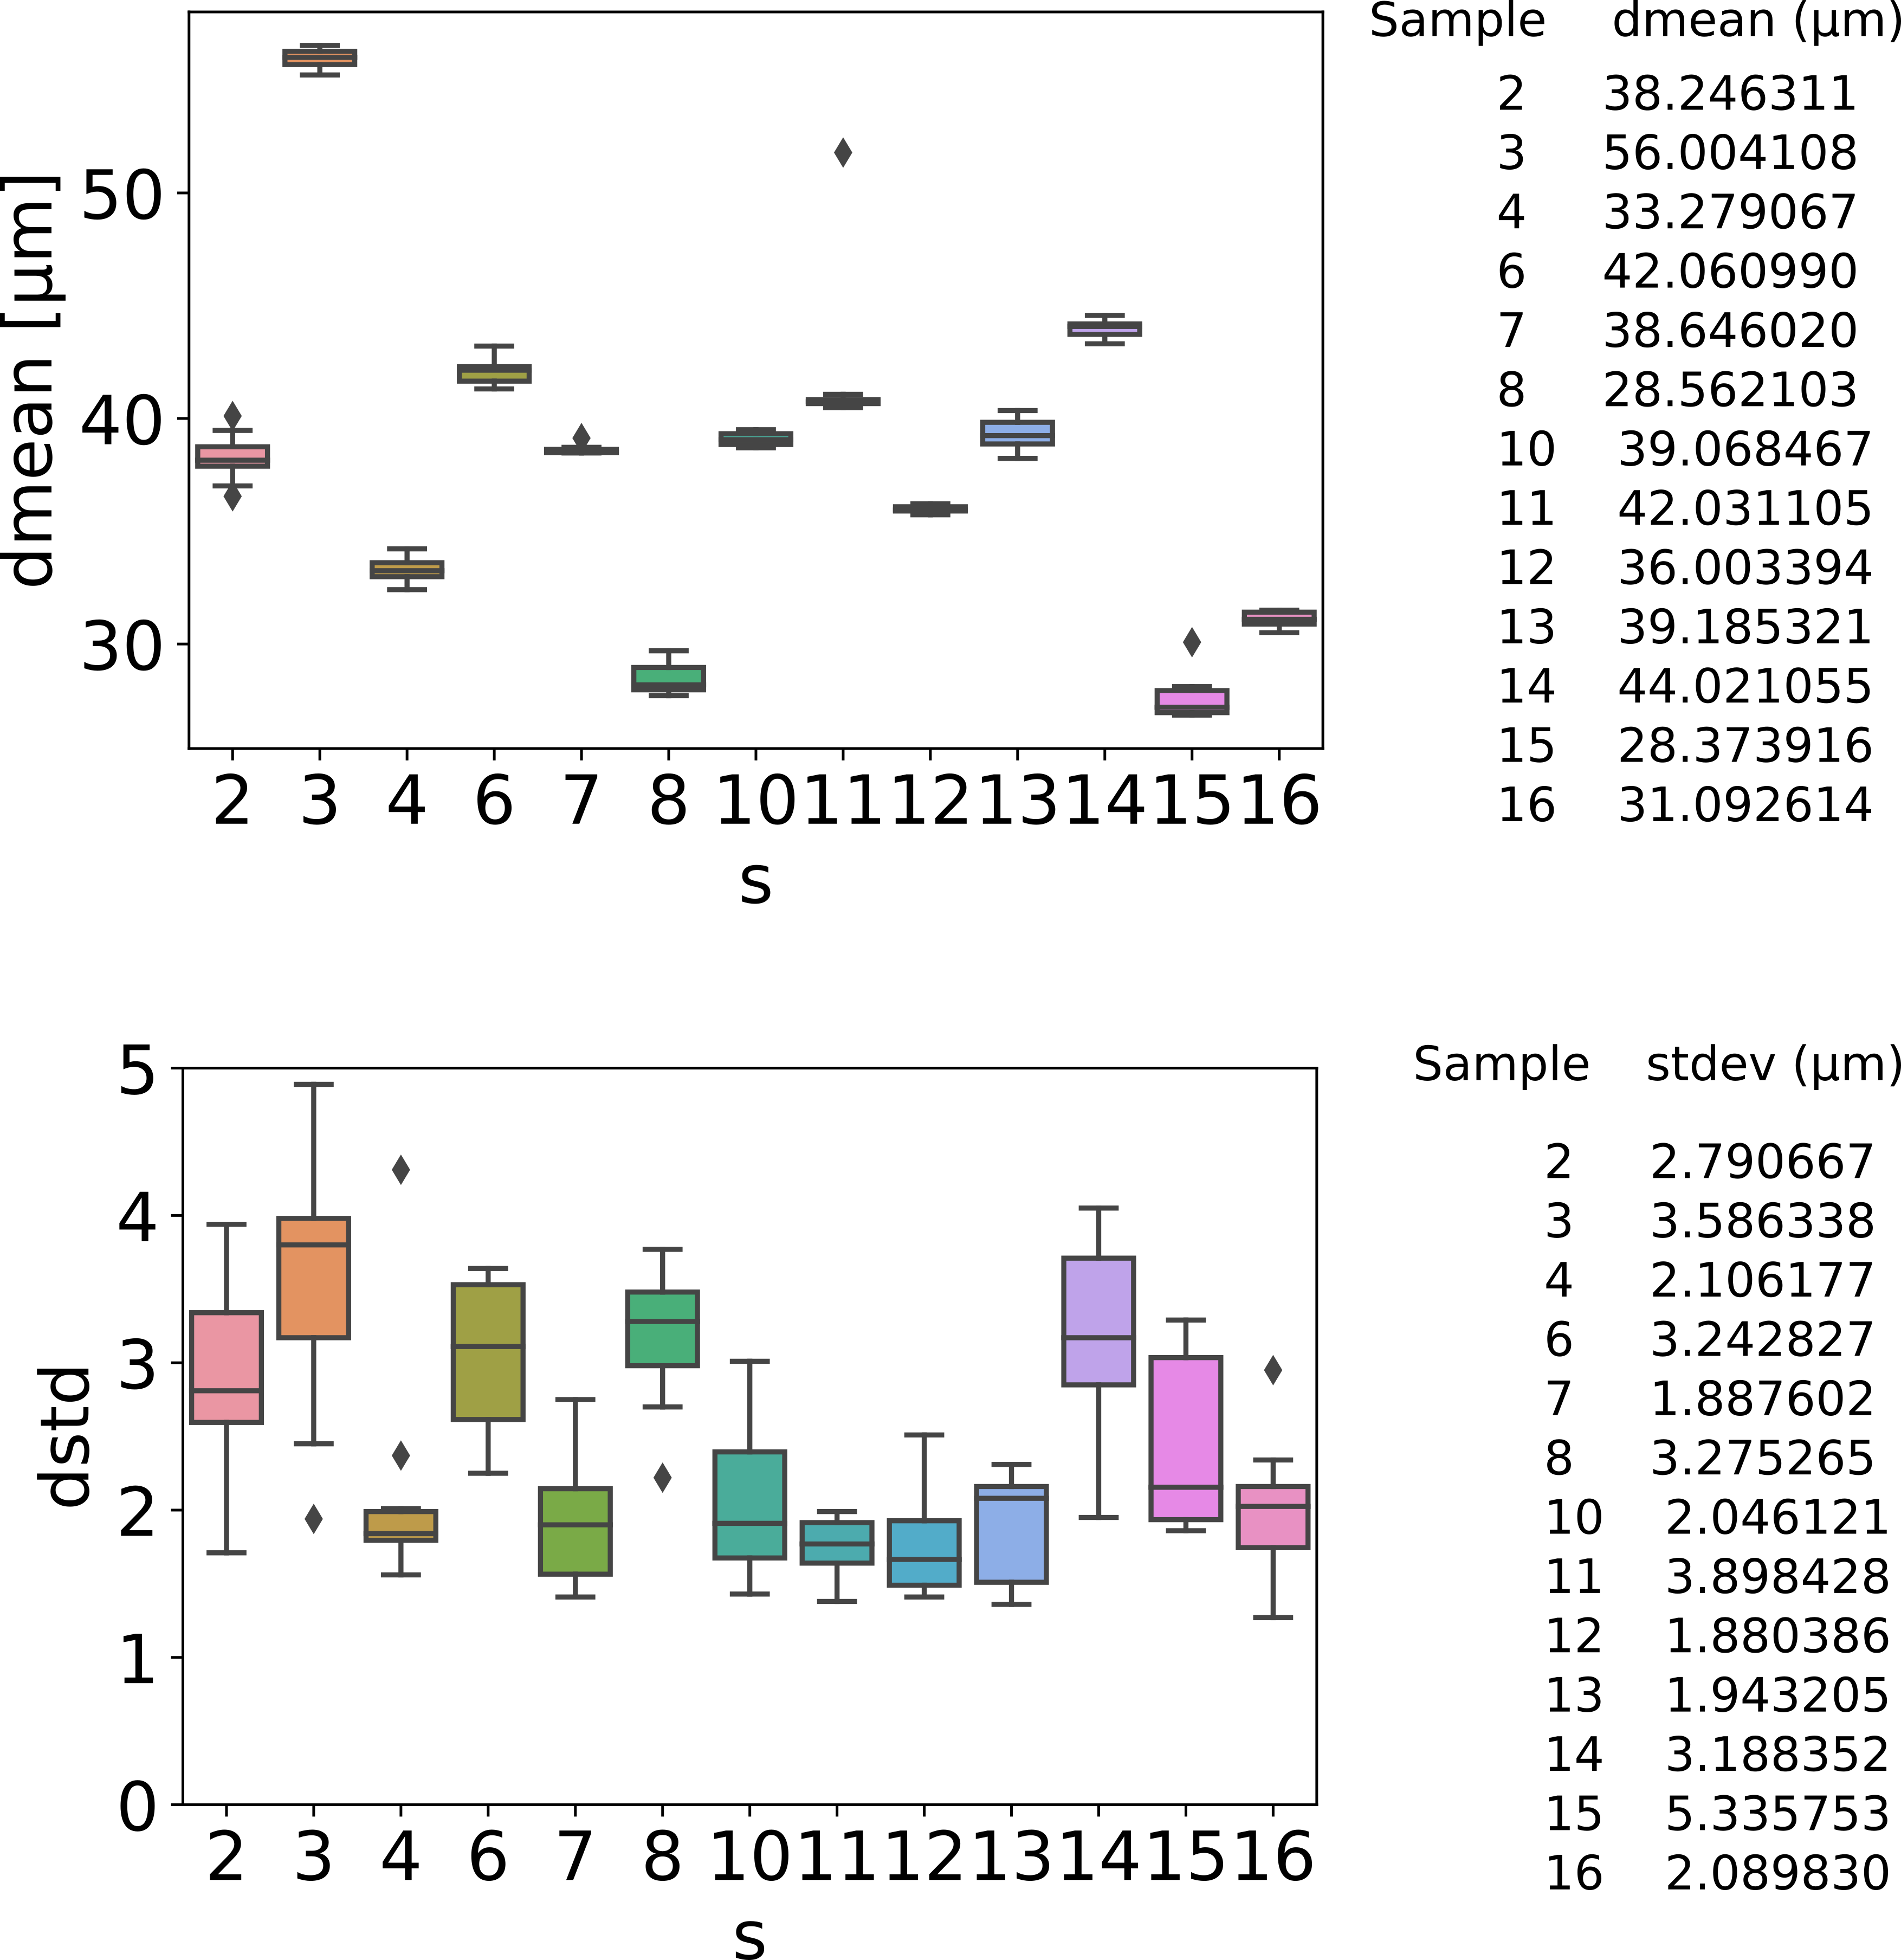
\includegraphics[width=\textwidth]{./ims/indrop_beaddata.png}
\caption[Hydrogel bead model dataset]{\textbf{Hydrogel bead model dataset.}}
\label{fig:indrop_model_data}
\end{figure}

\clearpage
\section{inDrop}

% \subsection{inDrop Chip Design}
% \label{app:indrop_chip_design}

% \begin{figure}[ht]
% \centerfloat
% 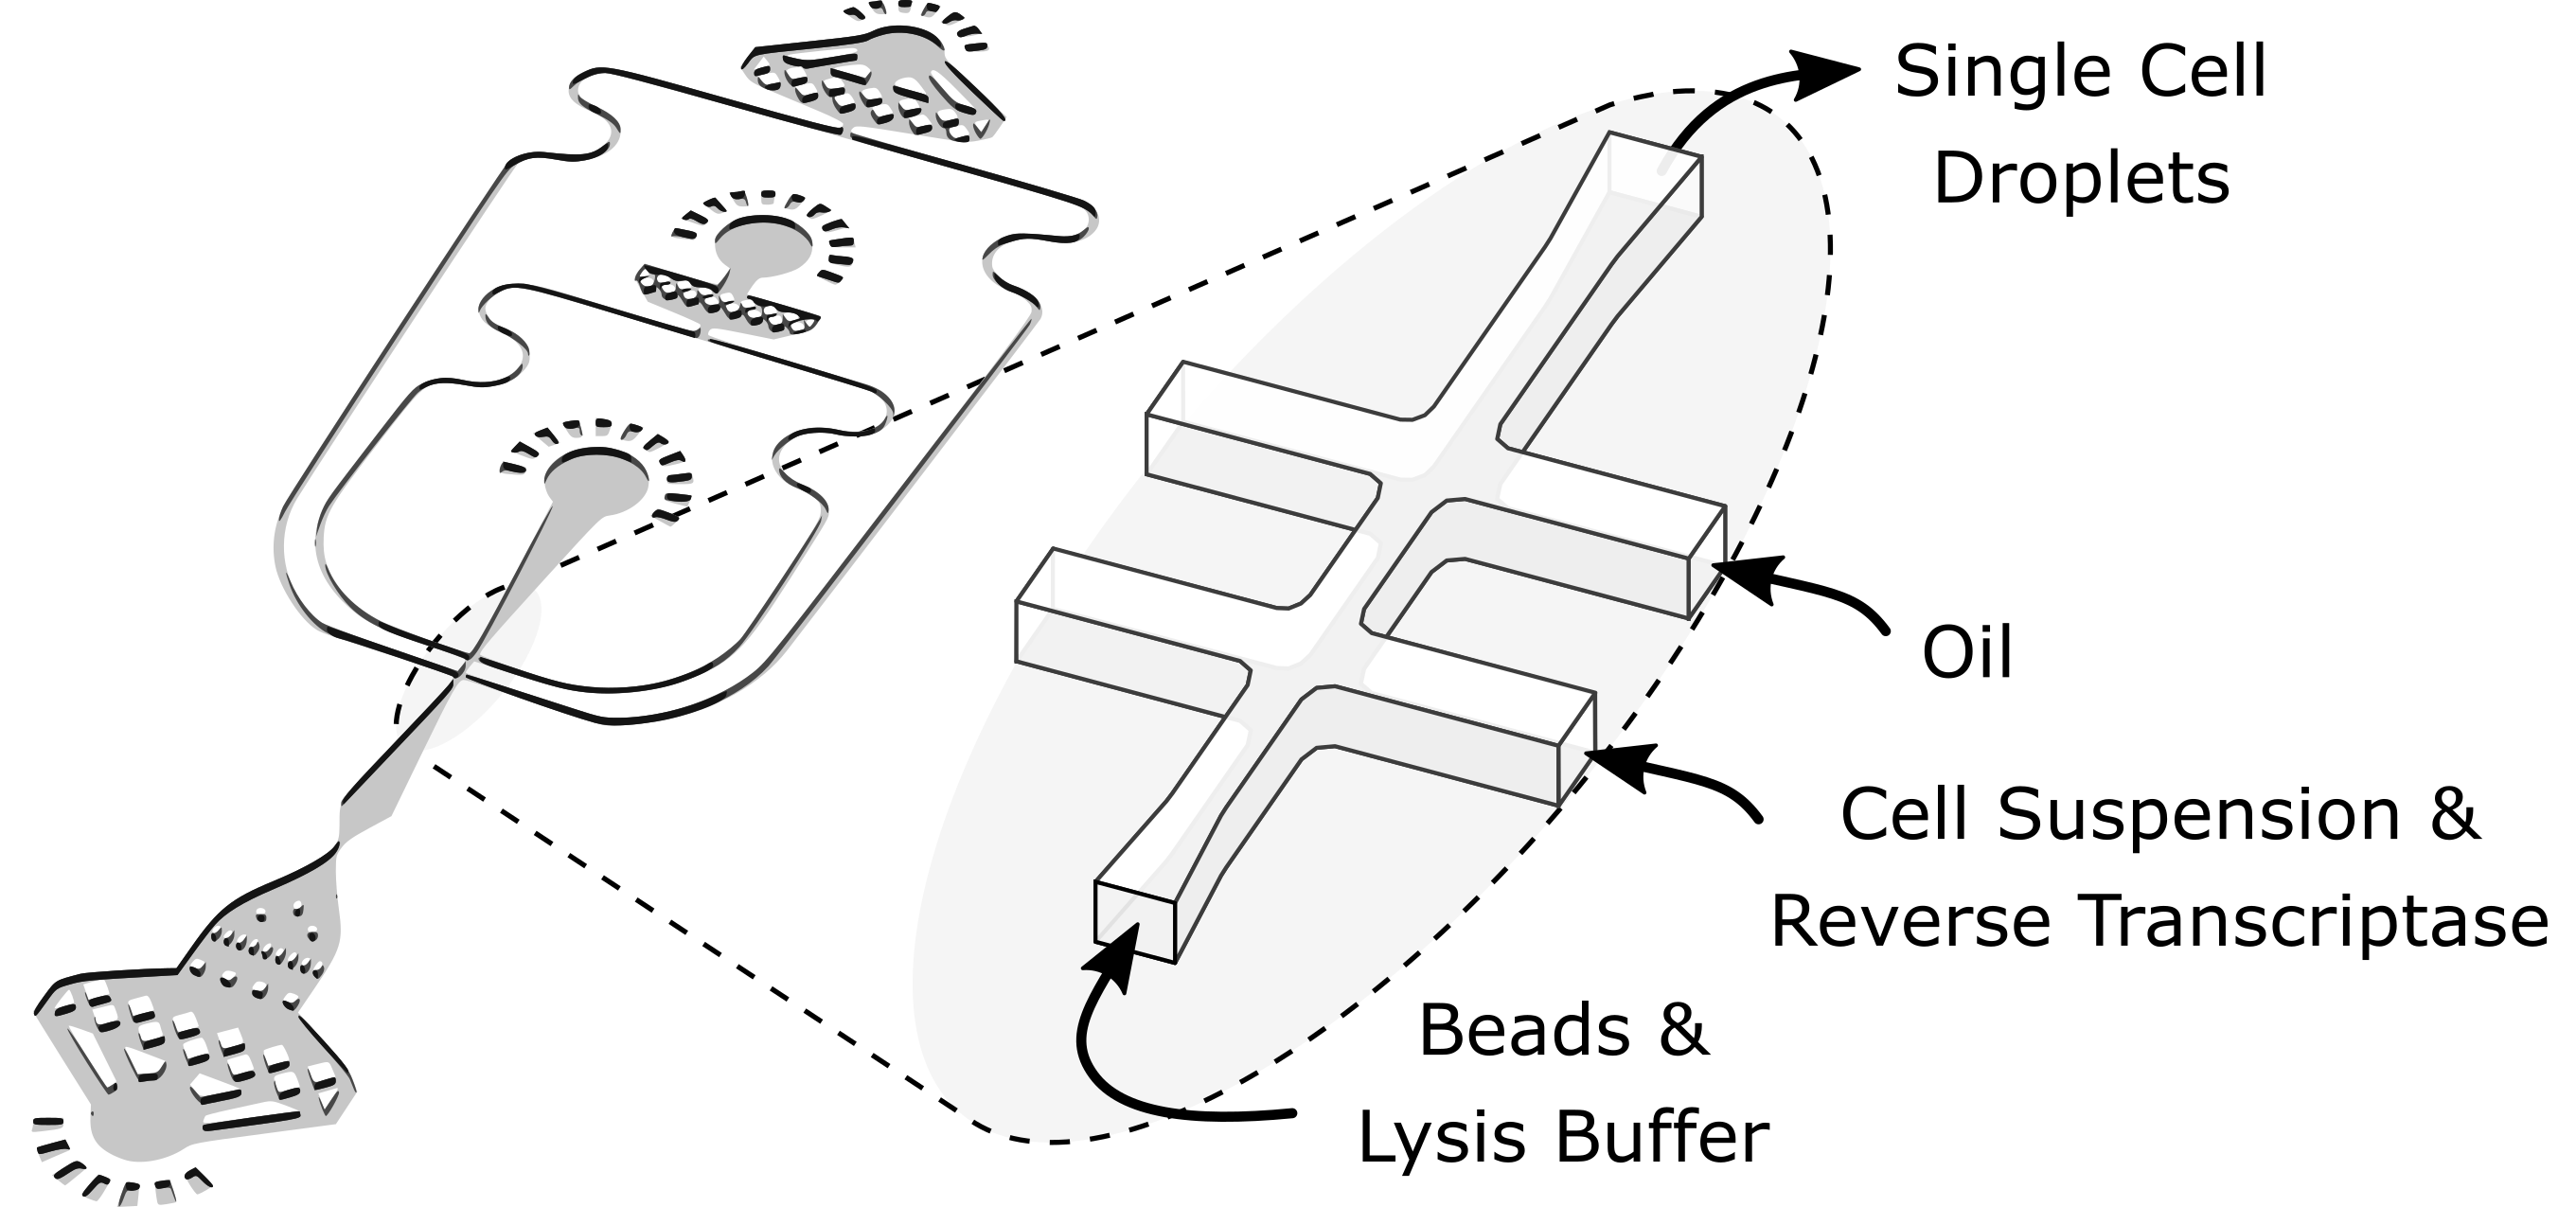
\includegraphics[width=\textwidth]{./ims/indrop_chip_zoom.png}
% \caption[inDrop Chip]{\textbf{inDrop Chip.}}
% \label{fig:app_indrop_chip_zoom}
% \end{figure}

\subsection{Failed Nextera Library Preparation Electropherogram}
\label{app:supp_nextera}

\begin{figure}[ht]
\centerfloat
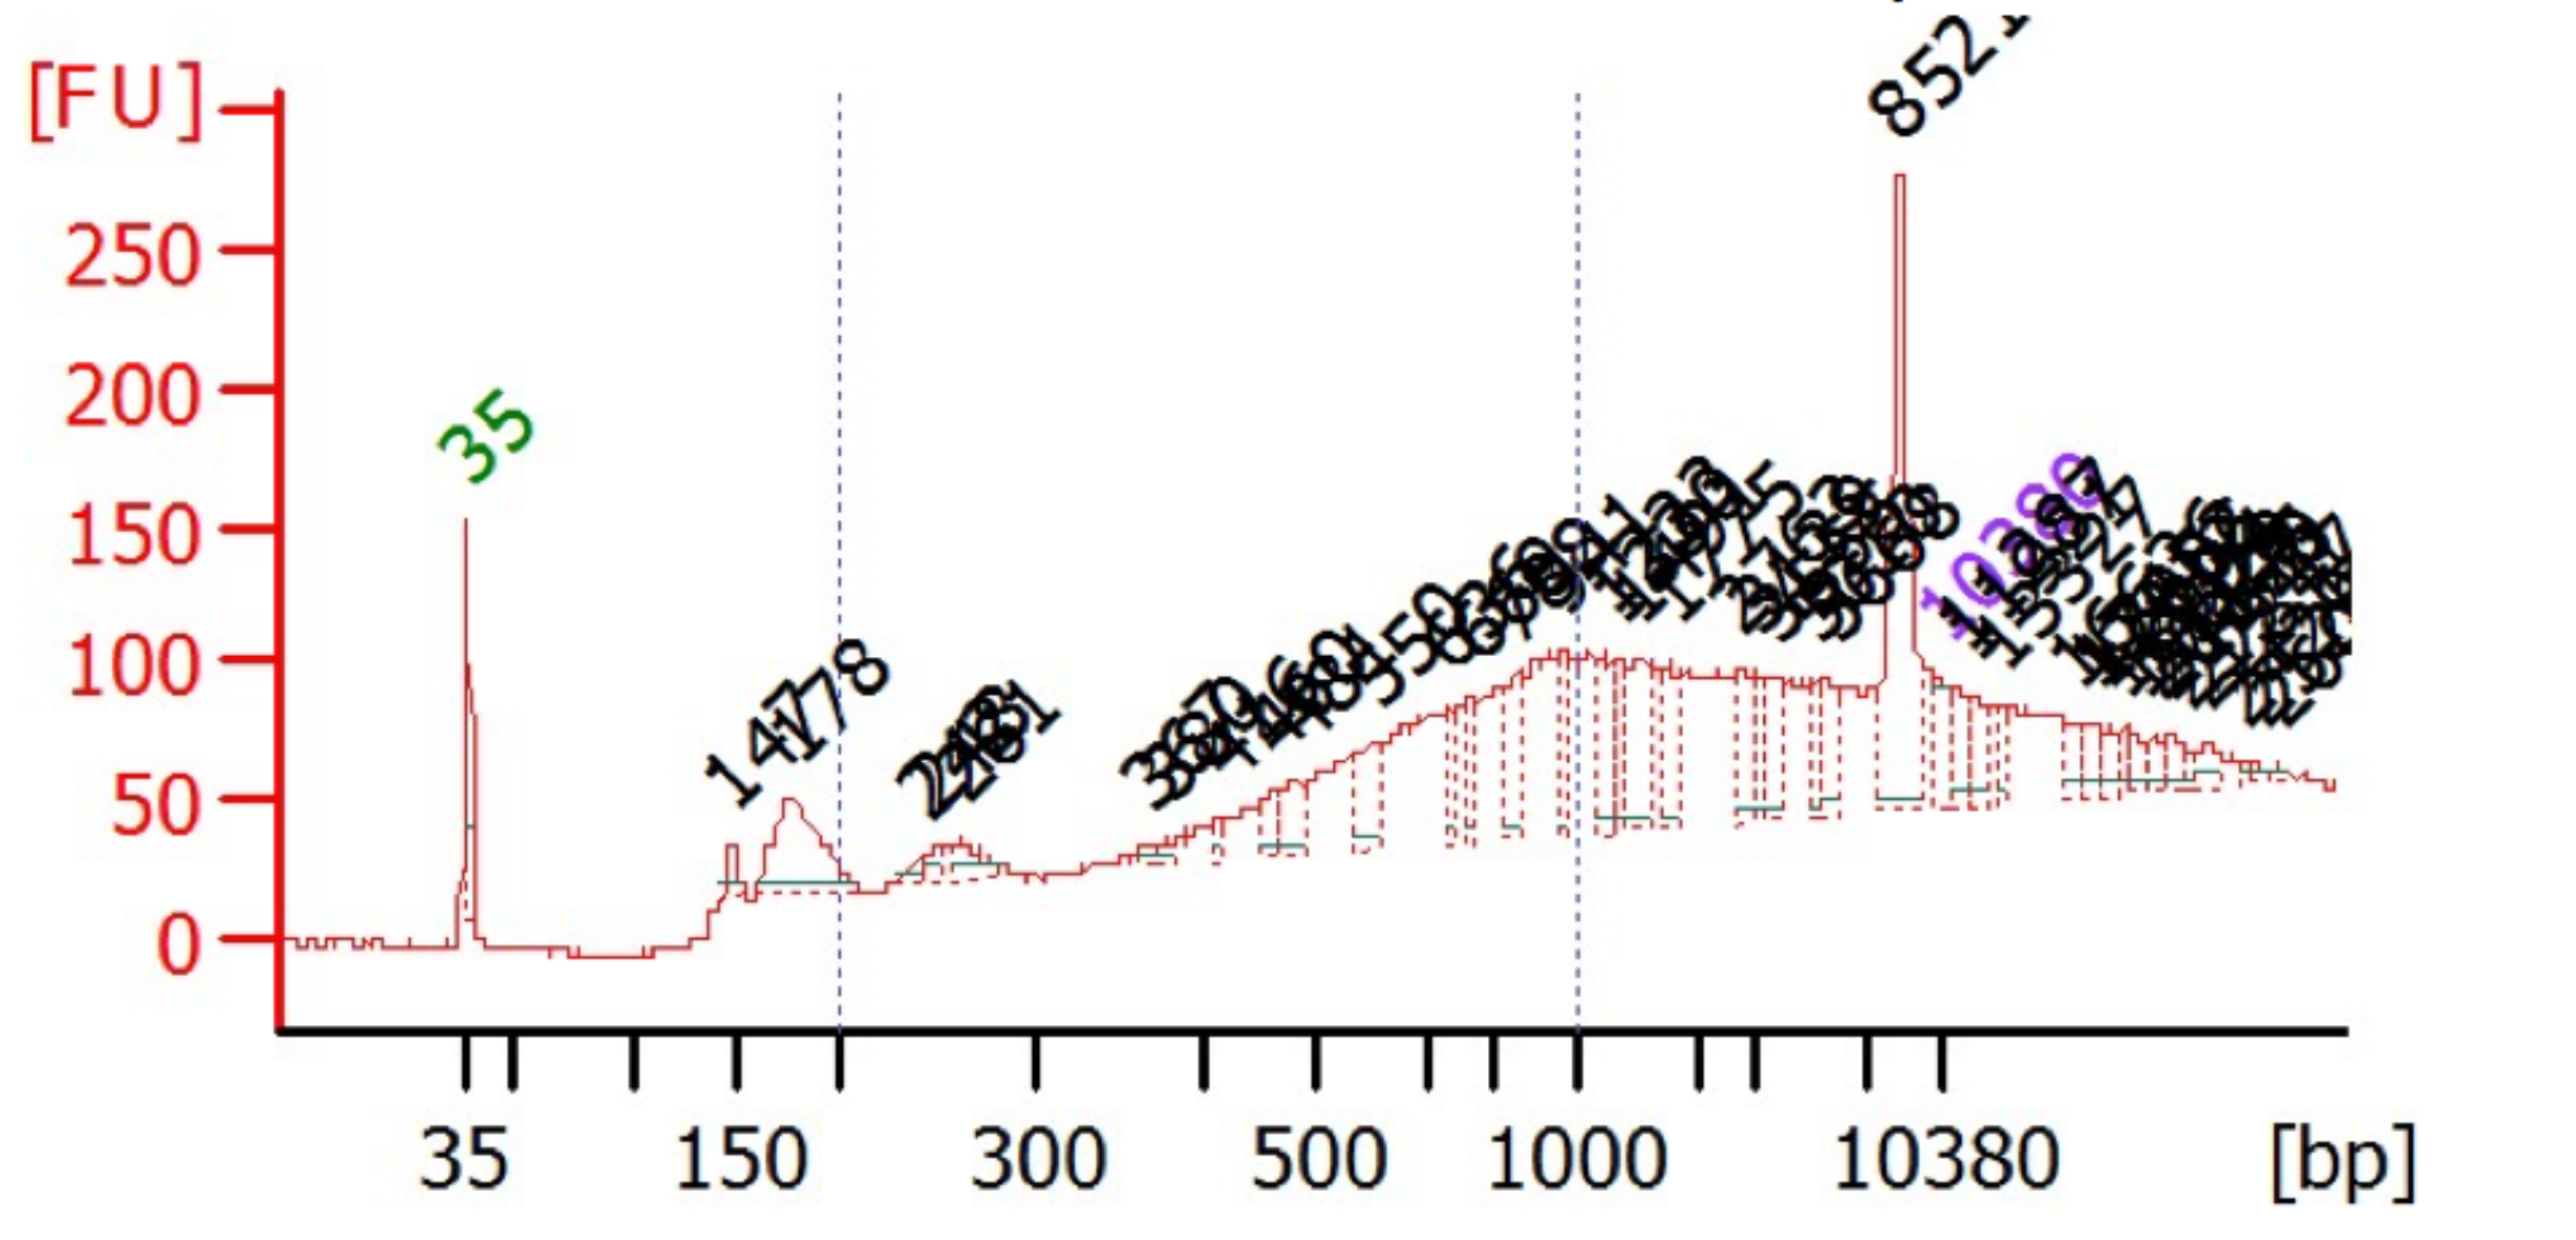
\includegraphics[width=\textwidth]{./ims/indrop_failednextera.png}
\caption[Failed Nextera Library Preparation electropherogram]{\textbf{Failed Nextera library preparation electropherogram.} The fragment distribution is too broad, too long and has an enrichment of small fragments, indicating residual primers. Generated by senior lab scientist.}
\label{fig:supp_nextera}
\end{figure}

\clearpage
\section{Sequencing}

\subsection{RNA-seq Datasets Correlations}
\label{app:supp_seq_ind_reseq_corr}
\begin{figure}[ht]
\centerfloat
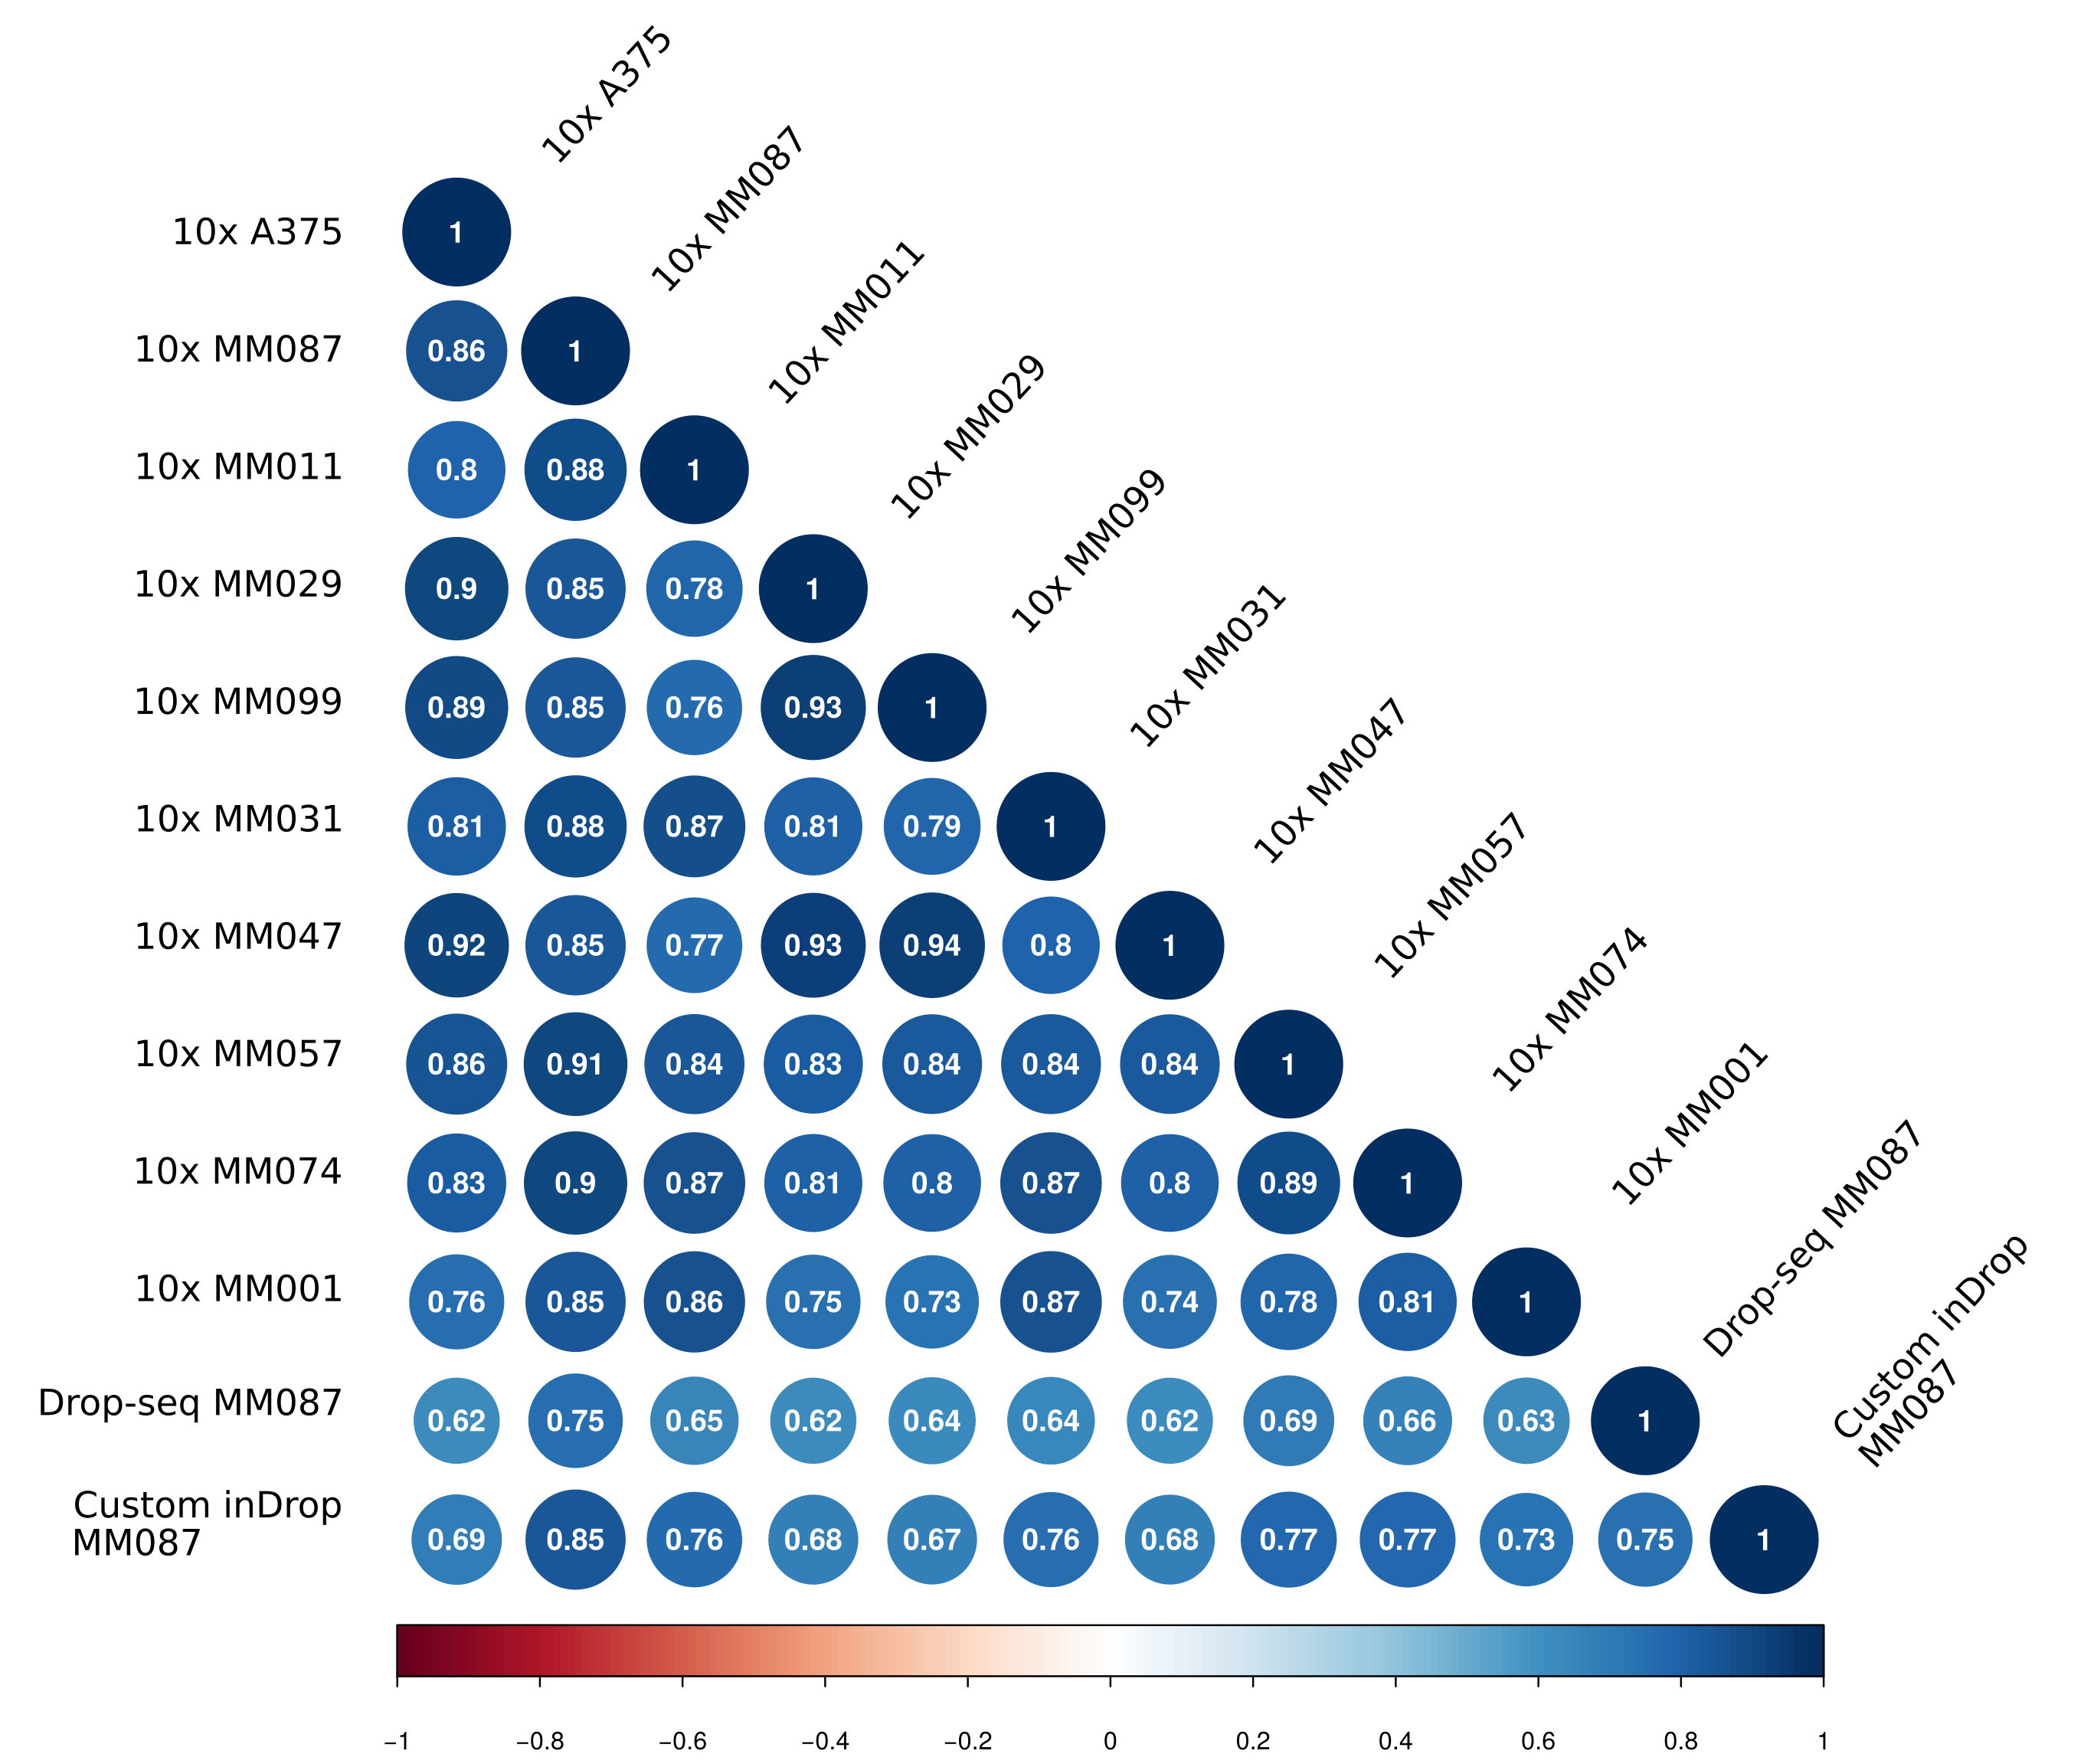
\includegraphics[width=\textwidth]{./ims/seq_ind_reseq_corr.png}
\caption[Correlations between different single-cell RNA-seq datasets]{\textbf{Correlation between different single-cell RNA-seq datasets.} Our inDrop MM087 dataset is slightly more correlated with the 10x MM087 dataset (p < 0.01).}
\label{fig:supp_seq_ind_reseq_corr}
\end{figure}

\clearpage
\subsection{Re-sequencing Run Gene Coverage}
\label{app:supp_seq_reseq_igv}
\begin{figure}[ht]
\centerfloat
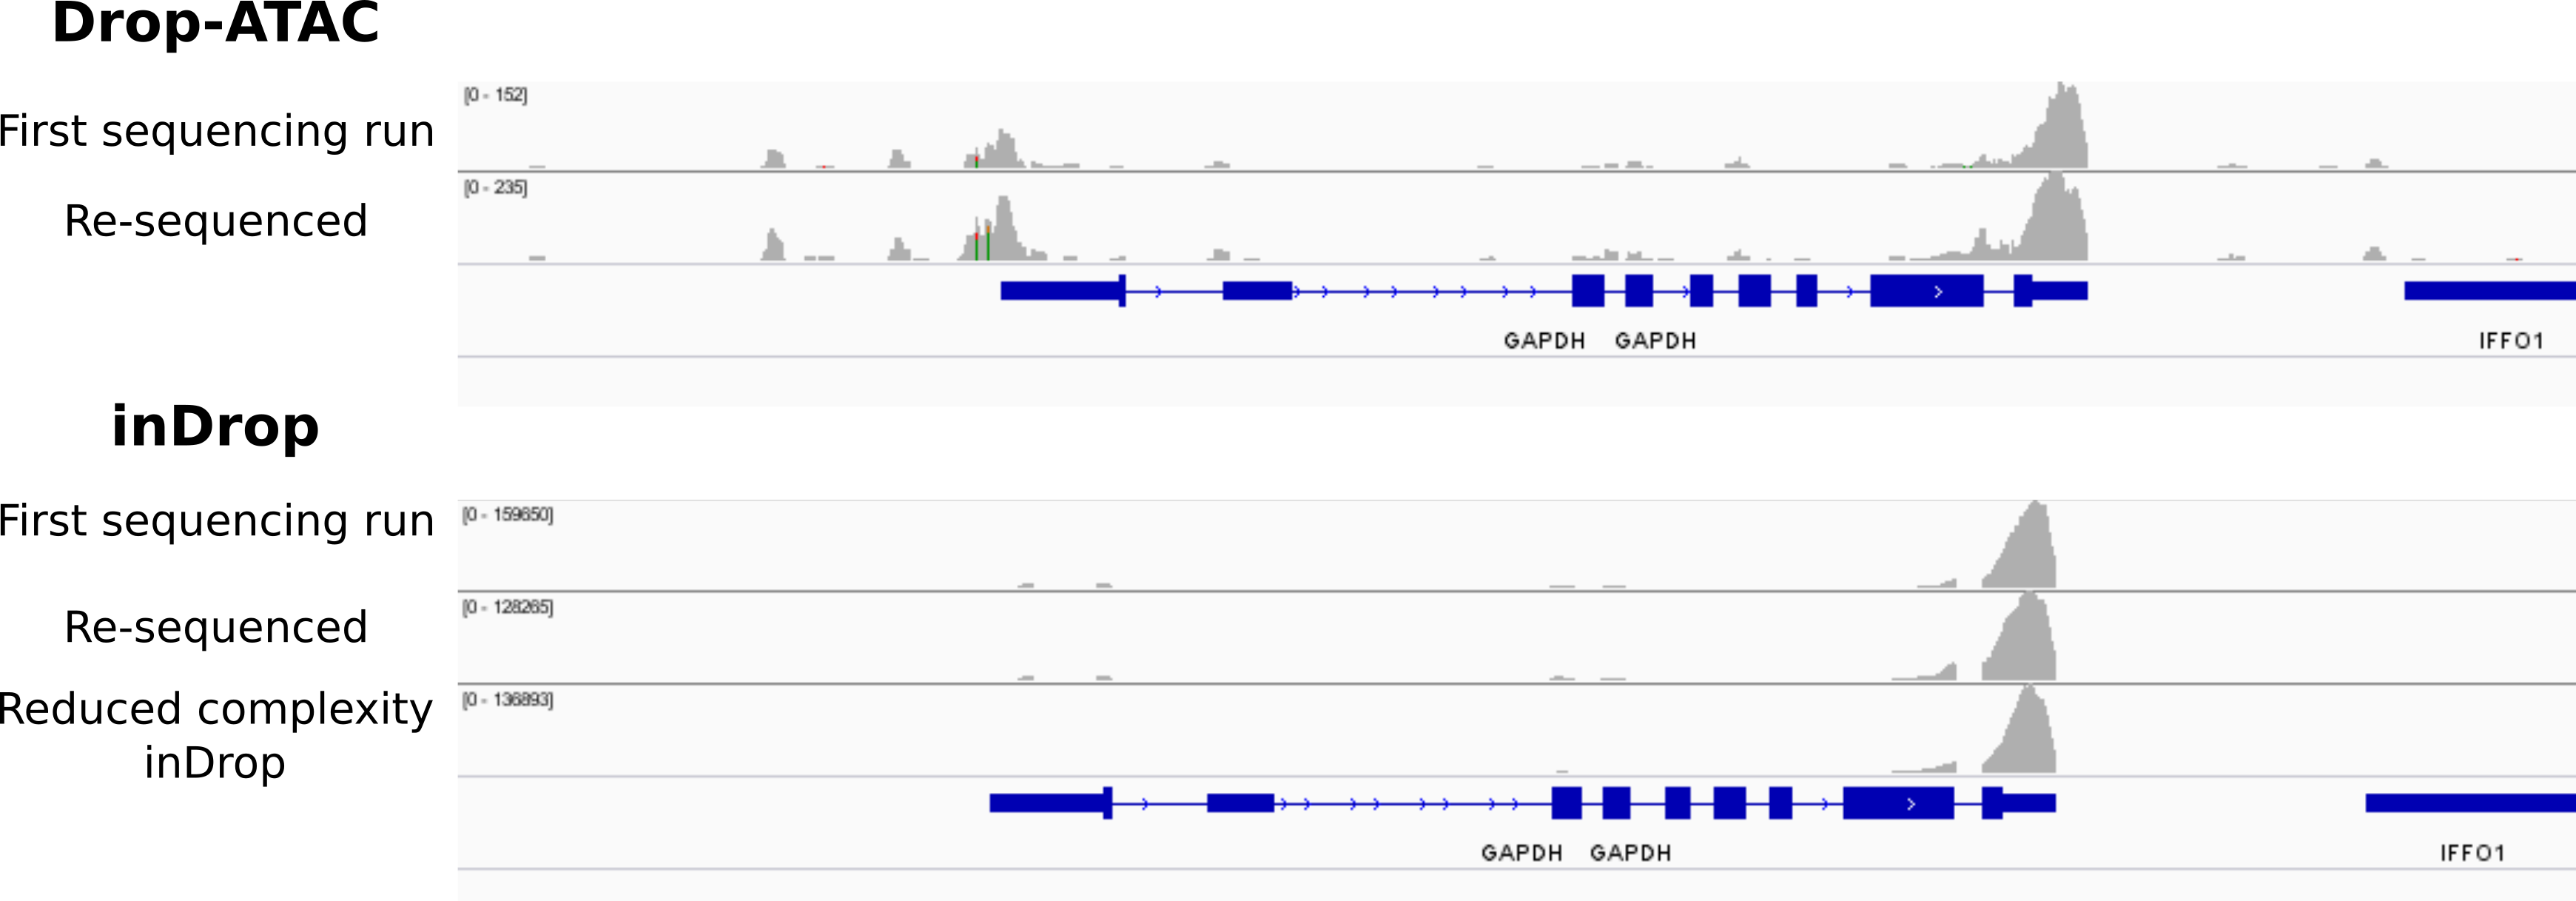
\includegraphics[width=\textwidth]{./ims/seq_reseq_igv.png}
\caption[Re-sequencing run gene coverage]{\textbf{Re-sequencing run gene coverage.} Gene coverage of reads, visualised in IGV.}
\label{fig:seq_reseq_igv}
\end{figure}

\clearpage

% \begin{figure}[ht]
% \centerfloat
% 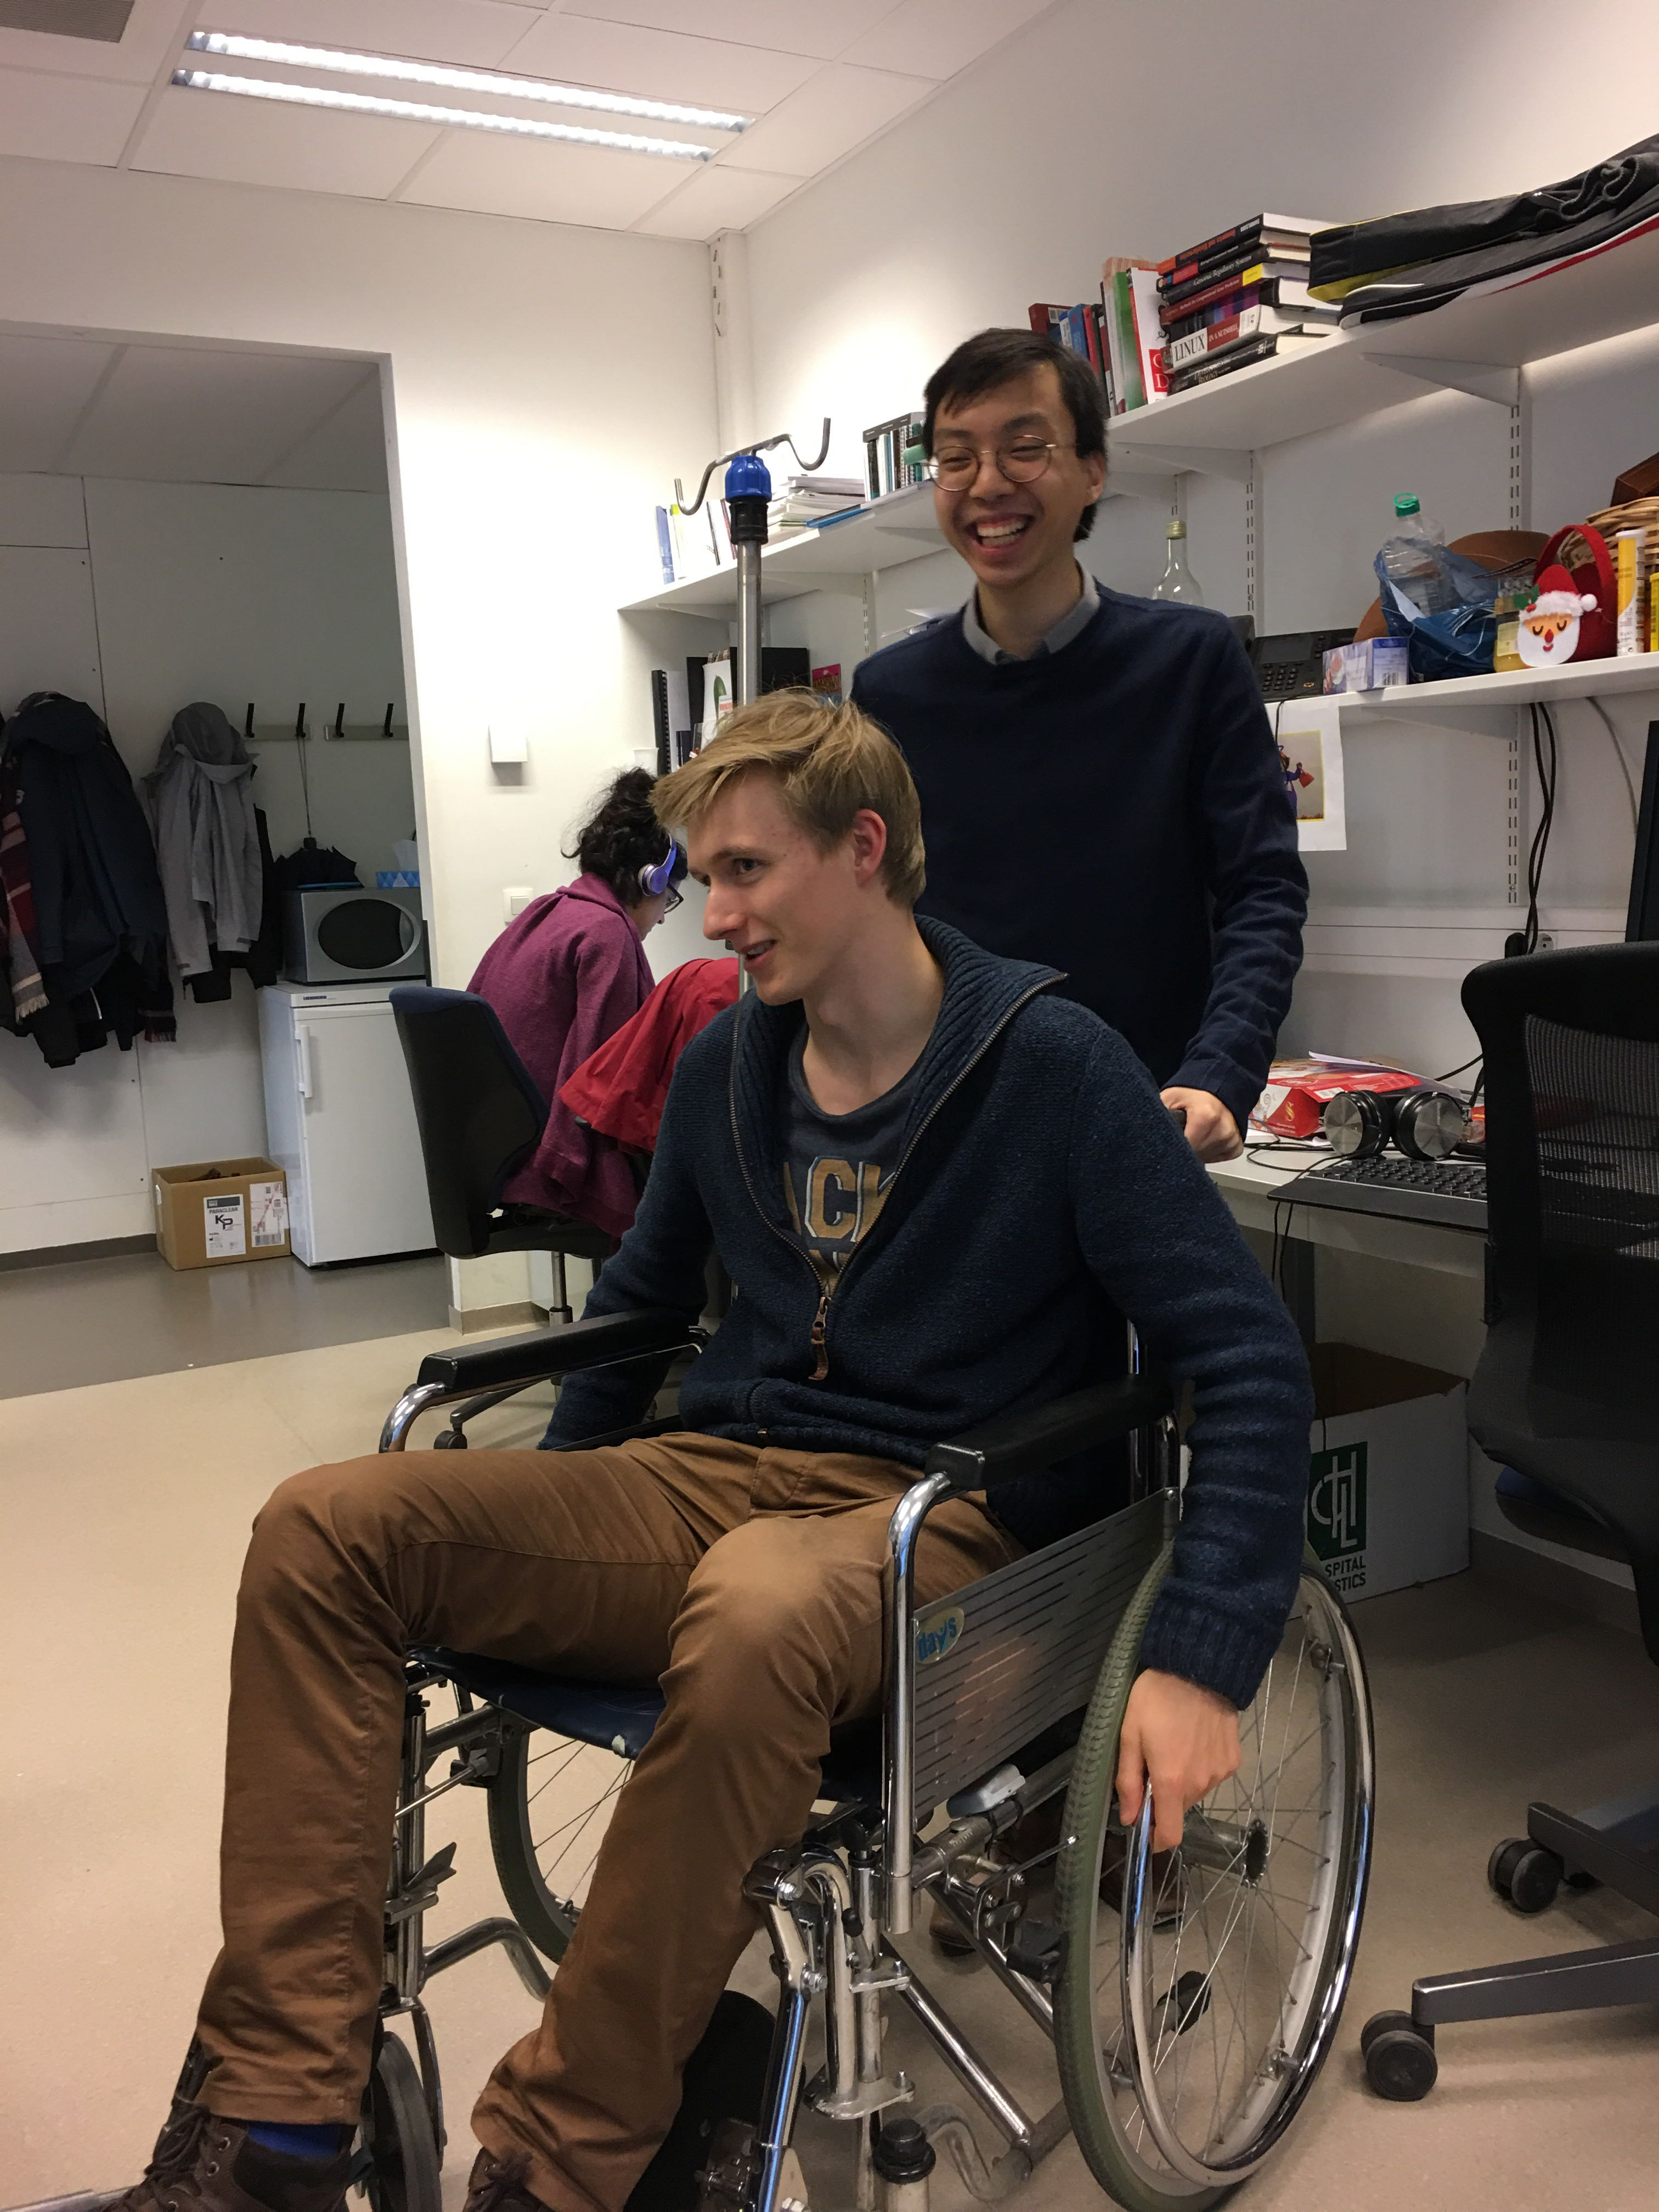
\includegraphics[width=\textwidth]{./ims/jbone.jpg}
% \caption[]{\textbf{A happy master student and his supervisor.}}
% \label{fig:}
% \end{figure}

\end{appendix}
